\documentclass[12pt,a4paper]{report}

\usepackage{geometry}
\geometry{a4paper, margin=2.5cm, headheight=14pt}
\usepackage{setspace}
\setstretch{1.85}
\usepackage{amsmath,amssymb,amsthm,mathtools}
\usepackage{graphicx}
\graphicspath{{figures/}}
\usepackage{booktabs}
\usepackage{array}
\usepackage{siunitx}
\sisetup{detect-all, range-phrase=--, range-units=single}
\usepackage{caption}
\usepackage{enumitem}
\usepackage{placeins}
\usepackage{tikz}
\usetikzlibrary{arrows.meta,positioning,calc,shapes.geometric,fit,backgrounds,decorations.pathreplacing}
\usepackage[hidelinks]{hyperref}
\usepackage[numbers,sort&compress]{natbib}

\sisetup{per-mode=symbol}
\DeclareSIUnit{\plato}{\textdegree P}
\DeclareSIUnit{\barg}{bar}

\captionsetup{font=small, labelfont=bf, skip=6pt}
\setlist[enumerate]{itemsep=2pt, topsep=4pt}
\setlist[itemize]{itemsep=2pt, topsep=4pt}

\newtheorem{assumption}{Assumption}[chapter]
\newtheorem{remark}{Remark}[chapter]

\newcommand{\degP}{^{\circ}\mathrm{P}}
\newcommand{\R}{\mathbb{R}}
\newcommand{\ud}{\mathrm{d}}
\newcommand{\ee}{\mathrm{e}}

\title{%
Research for Improving the Blending Accuracy of High-Gravity Beer\\
under Supply-Pressure Disturbance by Using Decoupled\\
Active Disturbance Rejection Control}
\author{Thesis draft\\[0.6em]\large Automatic control}
\date{2026}

\begin{document}
\pagenumbering{roman}
\maketitle
\thispagestyle{empty}

\begin{abstract}
\noindent
High-gravity brewing ferments a concentrated beer and then blends it, in line, with deaerated dilution water to the original extract required by the brand. On the blending skid considered in this thesis the actuators are three linear control valves: one on the high-gravity beer, one on the dilution water, and one on the outlet of the blend header. The measurements that are actually available for fast control are the liquid speeds in the three lines and the supply and header pressures. The original-extract analyser sits downstream of the mix point, behind a transport delay of about ten seconds.

Two control difficulties follow from that arrangement. The beer valve and the water valve are coupled by the header pressure, and the flow gain of each linear valve changes with the square root of the pressure drop, so a fixed-gain controller loses authority when a supply pressure falls. The extract loop, if it is closed on the analyser alone, is too slow to keep the blend inside the usual brewing tolerance of $\pm 0.05\degP$ during a recipe change or a supply disturbance.

This thesis proposes two techniques inside the active-disturbance-rejection framework. The first, pressure-manifold decoupled linear active disturbance rejection control, puts the installed interacting gain of each inlet valve into the observer as a known, measured coefficient. Supply pressure, header pressure and the steady coupling through the blend node are thereby removed from the total disturbance, while the small off-diagonal remainder, the relative-gain array element being only $1.11$, is left for the extended state observer. The second, valve-authority coordinated delay-compensated active disturbance rejection control, moves the outlet valve so that both inlet stems stay inside the linear portion of their stroke, and it closes the extract loop on a mass-balance soft sensor whose bias is corrected by the delayed analyser.

A first-principles numerical model of the skid, with valve stiction, sensor noise and the analyser lag, is used to estimate the two techniques against ratio proportional--integral control and against linear active disturbance rejection control with fixed nominal gains. Over a \SI{560}{s} campaign of supply steps, water-pressure oscillation, a brand change, a throughput increase, an unmeasured drift of the mother-beer extract and a loss of beer-valve capacity, the proposed pair reduces the integrated absolute extract error from \SI{81.4}{\plato\second} to \SI{52.4}{\plato\second} and the integrated absolute beer-flow error from \SI{316}{\cubic\metre\per\hour\second} to \SI{37.5}{\cubic\metre\per\hour\second}. The inlet stems remain away from the fully open seat in the cases where the fixed-gain designs saturate.
\end{abstract}

\chapter*{Principal symbols}
\addcontentsline{toc}{chapter}{Principal symbols}
\noindent
The symbols below are the ones used throughout the thesis. A symbol that is local to a derivation is defined where it appears. Pressures are gauge pressures unless an absolute pressure is stated.

\begin{center}
\begin{tabular}{@{}ll@{}}
\toprule
Symbol & Meaning \\
\midrule
$Q_h,Q_w,Q_b$ & Volumetric flow of high-gravity beer, dilution water and final beer \\
$v_h,v_w,v_b$ & Mean liquid speed in the three lines \\
$A_h,A_w,A_b$ & Internal cross-sectional area of the three pipes \\
$p_h,p_w$ & Supply pressure of beer and of dilution water \\
$p_m$ & Blend-header pressure \\
$p_d$ & Pressure downstream of the outlet valve \\
$x_h,x_w,x_b$ & Stem fractions of the three linear valves, in $[0,1]$ \\
$K_{v,h},K_{v,w},K_{v,b}$ & Metric flow coefficients of the three valves \\
$\rho_h,\rho_w,\rho_b$ & Densities of beer, water and the blend \\
$P_h$ & Original extract of the high-gravity beer \\
$P$ & Original extract of the blend \\
$P^\star$ & Original-extract setpoint \\
$R$ & Mass-consistent volumetric ratio $Q_w/Q_h$ \\
$\tau_v$ & Time constant of a valve positioner and actuator \\
$\tau_d$ & Transport delay from the mix point to the analyser \\
$b_0$ & Gain coefficient used by a linear extended state observer \\
$\omega_c,\omega_o$ & Controller bandwidth and observer bandwidth \\
$z_1,z_2$ & Extended-state estimates of the output and of the total disturbance \\
$\lambda_{11}$ & Diagonal element of the relative-gain array \\
\bottomrule
\end{tabular}
\end{center}

\tableofcontents
\listoffigures
\listoftables

\clearpage
\pagenumbering{arabic}

\chapter{Research of previous work}
\label{ch:review}

The blending step that closes a high-gravity brewery is a small plant with a large economic weight. A few seconds of wrong ratio put beer of the wrong strength into a bright-beer tank, and a valve that spends its life against the seat wears out and starts to stick. The actuators on the line studied here are ordinary linear control valves, and the fast measurements are liquid speeds and pressures. Everything that follows is an attempt to use those measurements well. This chapter sets out what is already known, in three parts. Section~\ref{sec:lit-tech1} reviews the control of coupled valve flows and the disturbance-rejection theory that the first technique builds on. Section~\ref{sec:lit-tech2} reviews delay compensation, inferential sensing and header-pressure coordination, which the second technique builds on. Section~\ref{sec:problem} states the blending problem in a form that those two techniques can be designed against.

\section{Research on coupled valve flow and disturbance decoupling}
\label{sec:lit-tech1}

\subsection{High-gravity beer and the dilution step}

High-gravity brewing is the practice of fermenting wort at an original extract above the extract of the beer that will be sold, and of restoring the sales gravity later by adding water \cite{stewart2010highgravity,kunze2014brewing,briggs2004brewing}. Stewart's account of the method puts the usual high-gravity range at \SIrange{15}{20}{\plato}, against a sales beer that may lie anywhere from a light lager near \SI{10}{\plato} to a full-bodied beer near \SI{13}{\plato} \cite{stewart2010highgravity}. The water added at the end of the process is carbon-filtered and stripped of oxygen, because oxygen picked up at this point shortens shelf life. The same idea appears in grain-whisky fermentation, where worts of \SIrange{18}{21}{\plato} are diluted after distillation rather than before it \cite{stewart2010highgravity,stewart1997recent}.

The brewing literature is mainly about yeast and flavour, and it is worth recording what it does and does not settle. High-gravity wort stresses yeast: vacuoles enlarge, the cell surface changes, and the uptake of maltotriose, the largest fermentable sugar, becomes incomplete \cite{stewart2010highgravity,boulton2001yeast,casey1984highgravity}. Foam stability falls, and the ester profile of the finished beer can drift away from the profile of a beer brewed at sales gravity \cite{stewart2010highgravity,briggs2004brewing}. Those are biological constraints. They fix the mother beer that the blender is allowed to receive. They do not say how the blender should move its valves when the supply pressure changes.

What the process books do fix is the dilution arithmetic \cite{kunze2014brewing,mebak2013wort,ebcanalytica}. Original extract is a mass fraction. If a mass flow $\dot{m}_h$ of high-gravity beer at original extract $P_h$ is mixed with a mass flow $\dot{m}_w$ of water, the original extract of the mixture is
\begin{equation}
\label{eq:plato-mass}
P = \frac{\dot{m}_h\, P_h}{\dot{m}_h + \dot{m}_w},
\end{equation}
because the water contributes no original extract. Volumetric flow meters and speed sensors report $Q = \dot{m}/\rho$, so the same balance written in the measured speeds is
\begin{equation}
\label{eq:plato-vol}
P = \frac{\rho_h v_h A_h\, P_h}{\rho_h v_h A_h + \rho_w v_w A_w}.
\end{equation}
Equation~\eqref{eq:plato-vol} is the soft sensor of Chapter~\ref{ch:design}. It is not an extra instrument. It is the mass balance evaluated on the speeds the skid already measures. The laboratory and the in-line analyser report the same quantity by density and sound velocity, on a sample that has travelled the length of the pipe after the mix point \cite{mebak2013wort,ebcanalytica,baker2016flow}.

Industrial skids close this balance with a ratio controller \cite{shinskey1996process,liptak2006handbook,seborg2016process}. Two flow loops track setpoints linked by $Q_w^\star = R\, Q_h^\star$, and a slow outer loop trims $R$ from the analyser. The ratio is applied to the setpoints rather than to the measured beer flow, which avoids a positive feedback from beer-flow noise into the water setpoint \cite{shinskey1996process}. That structure is the right cascade. Its weakness on this plant is the gain inside each flow loop, not the decision to use a ratio.

\subsection{The linear valve and the installed pressure drop}

A control valve for clean beer or deaerated water on a sanitary skid is typically a globe or a diaphragm valve with a linear inherent characteristic and a pneumatic positioner \cite{fisher2005valve,iec60534general,iec60534}. The inherent characteristic is the flow curve measured at a constant pressure drop. For a linear valve the fraction of the rated flow equals the stem fraction $x\in[0,1]$,
\begin{equation}
\label{eq:inherent}
f(x) = x.
\end{equation}
The sizing equation used for incompressible liquids in IEC~60534-2-1 relates the volumetric flow in cubic metres per hour to the pressure drop in bar and to the specific gravity \cite{iec60534,fisher2005valve},
\begin{equation}
\label{eq:kv}
Q = K_v\, x\, \sqrt{\frac{\Delta p}{\rho/1000}}.
\end{equation}
Here $K_v$ is the metric flow coefficient, the flow of water in \si{\cubic\metre\per\hour} that the fully open valve passes at a pressure drop of \SI{1}{\barg}. The square-root dependence is the whole difficulty. A controller tuned at one pressure drop is mistuned at another, in proportion to the square root of the ratio of the drops.

The drop across an inlet valve is not an independent input. It is the difference between a supply pressure, set by a tank head or a pump, and the header pressure $p_m$, which is common to both inlet valves and is itself set by the outlet valve. For the beer valve,
\begin{equation}
\label{eq:dp-beer}
\Delta p_h = p_h - p_m.
\end{equation}
Differentiating \eqref{eq:kv} at fixed stem position gives the pressure sensitivity
\begin{equation}
\label{eq:pressure-sensitivity}
\frac{\partial Q_h}{\partial p_m} = -\frac{Q_h}{2(p_h-p_m)}.
\end{equation}
A rise in header pressure reduces beer flow and water flow together, and it increases the flow through the outlet valve. The three valves therefore meet a single algebraic constraint. On a liquid-full line the accumulation in the header pipe is negligible on the time scale of a positioner, so
\begin{equation}
\label{eq:node}
Q_h(x_h,p_h,p_m) + Q_w(x_w,p_w,p_m) - Q_b(x_b,p_m,p_d) = 0.
\end{equation}
Equation~\eqref{eq:node} defines $p_m$ as an implicit function of the three stems and the three boundary pressures. The gain that a flow controller actually sees is not the partial derivative at frozen $p_m$. It is the total derivative along \eqref{eq:node}.

Let $S_h = Q_h/(2\Delta p_h)$, $S_w = Q_w/(2\Delta p_w)$ and $S_b = Q_b/(2\Delta p_b)$, all positive. Implicit differentiation of \eqref{eq:node} produces the installed gains used in Chapter~\ref{ch:design}. The diagonal beer gain is smaller than the partial gain $Q_h/x_h$ by the factor $(S_w+S_b)/(S_h+S_w+S_b)$, because part of any extra beer flow is absorbed by a rise in $p_m$. This is the installed characteristic discussed in the valve handbooks \cite{fisher2005valve,iec60534}. Figure~\ref{fig:installed} sketches the distinction. The inherent line is straight. The installed line bends, and it moves when the supply pressure moves.

\begin{figure}[htbp]
\centering
\begin{tikzpicture}[x=5.2cm,y=4.2cm,>=Stealth]
  \draw[->] (0,0) -- (1.15,0) node[below] {stem fraction $x$};
  \draw[->] (0,0) -- (0,1.15) node[left] {relative flow};
  \draw[thick] (0,0) -- (1,1) node[right] {inherent};
  \draw[thick, dashed] plot[smooth] coordinates {(0,0) (0.25,0.18) (0.5,0.42) (0.75,0.72) (1,1)};
  \node[right] at (1,0.92) {installed};
  \draw[thick, dotted] plot[smooth] coordinates {(0,0) (0.3,0.12) (0.6,0.28) (0.85,0.48) (1,0.62)};
  \node[right] at (1,0.55) {installed, lower $\Delta p$};
  \draw[decorate, decoration={brace, amplitude=4pt}] (0.32,0.05) -- (0.72,0.05);
\end{tikzpicture}
\caption{Inherent and installed flow curves of a linear valve. The preferred operating window is the middle of the stroke, where the installed gain is finite and a small stick band is a small fraction of the flow.}
\label{fig:installed}
\end{figure}

Bristol's relative-gain array is the standard scalar summary of this interaction \cite{bristol1966rga,skogestad2005multivariable}. For a two-by-two gain matrix $G$ the diagonal relative gain is
\begin{equation}
\label{eq:rga}
\lambda_{11} = \frac{1}{1 - \dfrac{G_{12}G_{21}}{G_{11}G_{22}}}.
\end{equation}
A value near one means that a decentralised controller, one loop per valve, does not fight its neighbour in the steady state. A value far from one means that a decoupler, or a truly multivariable controller, is required \cite{skogestad2005multivariable,seborg2016process}. The calculation in Section~\ref{sec:problem} gives $\lambda_{11}=1.11$ at the design point of this skid. The interaction is real, and it is visible in the off-diagonal gains, but it is not large enough to justify inverting $G$. Inverting a matrix that is uncertain by the amount of a sticky valve amplifies that uncertainty \cite{skogestad2005multivariable,morari1989robust}. The appropriate decentralised action is to put the correct diagonal installed gain into each loop and to let feedback remove the off-diagonal remainder. That is the classical Bristol recommendation, and it is the structural choice of the first technique.

\subsection{What a fixed-gain flow loop cannot absorb}

Process-control practice tunes the flow loops with a proportional--integral controller \cite{ziegler1942optimum,rivera1986imc,skogestad2003simc,astrom2006advanced}. For a first-order valve, the SIMC rules of Skogestad give a proportional gain inversely proportional to the process gain and an integral time equal to the valve time constant, provided the closed-loop time constant is chosen a little slower than the positioner \cite{skogestad2003simc}. The rules are explicit, and they are the baseline in Chapter~\ref{ch:estimate}. They have two limits that matter here.

The first limit is the gain schedule hidden inside \eqref{eq:kv}. SIMC is derived at one linearisation. When $p_h$ falls, $\Delta p_h$ falls and the process gain falls with the square root. A proportional gain that was correct becomes too small, the loop slows down, and the stem runs toward the open stop in an attempt to recover the flow. Once the stem is above about $0.9$, the remaining travel produces little extra flow and the positioner works in the region where seal friction is the least repeatable \cite{fisher2005valve,choudhury2005modelling}. Bialkowski's survey of industrial loops put the fraction of loops that perform well below one third, and named valve friction as a principal cause \cite{bialkowski1993dreams}. H\"agglund's performance monitor detects the same oscillation from the controller output alone \cite{hagglund1995monitor}. The quantitative stiction models of Choudhury, Thornhill and Shah, and the later detection methods collected by Jelali and Huang, describe a stick band and a slip jump \cite{choudhury2005modelling,choudhury2008stiction,jelali2010stiction}. A positioner reduces the apparent band, but it does not remove it. A controller that continually nudges a valve inside the band produces no flow change and then a jump.

The second limit is dynamic coupling during the transient. Even if $\lambda_{11}$ is near one, a fast move of the water valve changes $p_m$ before the beer loop has finished its own correction. Ratio control on setpoints keeps the commands in proportion. It does not keep the delivered flows in proportion during that window \cite{shinskey1996process,luyben1990process}. The extract error is exactly the error in that proportion, through \eqref{eq:plato-vol}.

Model predictive control can be written for the same plant, and the industrial record of predictive control on constrained multivariable processes is strong \cite{qin2003mpc,bequette2003process,ogunnaike1994process,stephanopoulos1984chemical}. A predictive controller needs a model that is kept up to date, a horizon long enough to cover the analyser delay, and a quadratic program inside the cycle time of a flow loop. On a skid whose fast loops are flow loops with a one-second time scale, that machinery is difficult to justify when the dominant uncertainty is a pressure that is already measured. The disturbance-rejection route uses the measurement directly and leaves the unmeasured remainder to an observer.

\subsection{From disturbance accommodation to the extended state}

The idea of estimating a disturbance and cancelling it is older than active disturbance rejection. Johnson's disturbance-accommodating control augments the plant with a model of a disturbance that is generated by a known exosystem, and then estimates that state \cite{johnson1971accommodation}. The internal-model principle of Francis and Wonham gives the corresponding structural result: a regulator that rejects a disturbance asymptotically must contain a model of the dynamics that generate it \cite{francis1976internal}. Ohishi and co-workers built the same idea into a disturbance observer for a motor, subtracting an estimated load torque from the current command \cite{ohishi1987microprocessor}. Schrijver and van Dijk later showed the equivalence of several of these observers for rigid mechanical plants and gave design conditions \cite{schrijver2002disturbance}. Chen, Yang, Guo and Li reviewed the whole family and separated the methods by what they assume about the disturbance channel \cite{chen2016dobc,li2014dobc}.

Active disturbance rejection, introduced by Han and put into bandwidth form by Gao, makes a sharper modelling choice \cite{han1998adrc,han2008book,han2009pid,gao2003scaling,gao2006paradigm}. Every effect that is not the chosen nominal chain of integrators is collected into one signal, the total disturbance, and that signal is treated as an extra state. For a first-order loop the plant is written
\begin{equation}
\label{eq:first-order-total}
\dot{y} = f(y,d,t) + b\, u,
\end{equation}
where $u$ is the valve command, $y$ is the measured flow or pressure, $b$ is a gain, and $f$ contains valve friction, density error, coupling, and the mismatch $b_{\mathrm{true}}-b$. The extended state is $x_2=f$, with $\dot{x}_2=h$ treated as unknown but bounded. The linear extended state observer of Gao is
\begin{align}
\dot{z}_1 &= z_2 + b_0 u + 2\omega_o (y-z_1), \label{eq:leso1}\\
\dot{z}_2 &= \omega_o^2 (y-z_1), \label{eq:leso2}
\end{align}
and the control that cancels $z_2$ and assigns the bandwidth $\omega_c$ is
\begin{equation}
\label{eq:ladrc-u}
u = \frac{\omega_c(r-z_1) - z_2}{b_0}.
\end{equation}
The two numbers $\omega_c$ and $\omega_o$ replace the three PID numbers, which is the practical content of the bandwidth parameterisation \cite{gao2003scaling}. Herbst's simulation study showed that a practitioner can obtain, with those two numbers, the kind of transient that a carefully tuned PID gives, and a better recovery after a load step \cite{herbst2013simulative}. Plant trials in thermal power stations have since made the same comparison on steam temperature and on the transition from an existing PID \cite{sun2016tuning,wu2021transition}.

The theoretical support is now substantial. Guo and Zhao proved convergence of the extended state observer for a class of nonlinear uncertain systems, and collected the theory in monograph form \cite{guo2011convergence,guo2016book}. Huang and Xue set out the methodology and the separation between the observer time scale and the controller time scale \cite{huang2014methodology}. Xue and Huang gave performance bounds for uncertain linear plants \cite{xue2015performance}. Zheng, Gao and Gao validated the observer experimentally and showed that the estimate $z_2$ tracks a real load when $\omega_o$ is high enough and the sampling rate is several times $\omega_o$ \cite{zheng2012validation}. Sira-Ram\'irez and co-workers connected the same observer to differential flatness and demonstrated it on a permanent-magnet motor \cite{sira2017adrc,sira2014pmsm}. Gao's later essay argued that disturbance rejection, rather than model following, is the central job of a feedback loop in industry \cite{gao2014centrality}. Madonski and co-workers rewrote the two-degree-of-freedom form as a single error-driven block that fits an industrial function-block diagram \cite{madonski2019error}.

Two limitations of the plain observer matter for a valve.

The gain $b_0$ is a design choice, and a bad choice is expensive. If $b_0$ is far from the true $b$, the quantity $z_2$ must carry $(b-b_0)u$ as well as the physical disturbance. Fu and Tan showed how to fold known plant information into the observer so that $z_2$ carries only the unknown part, and they gave tuning rules for that case \cite{fu2016tuning}. Tan and Fu showed that linear active disturbance rejection for a first-order or second-order plant is an internal-model controller with a particular filter, which explains both its robustness and the noise penalty of a high $\omega_o$ \cite{tan2016imc,rivera1986imc}. On the blending skid the dominant known part is \eqref{eq:kv} evaluated at the measured pressures. Leaving that part inside $f$ forces $\omega_o$ up, and the higher observer gain passes flow-meter noise into the stem command. Putting it into $b_0(t)$ is exactly the use of known plant information that Fu and Tan recommend, specialised to a valve whose gain is a measured pressure.

The second limitation is noise. A linear observer of bandwidth $\omega_o$ differentiates, in effect, with a gain that grows as $\omega_o^2$ for the disturbance channel. Madonski and Herman surveyed the modifications that reduce this cost \cite{madonski2015survey}. \L{}akomy and Madonski cascade two observers so that a high bandwidth can be used without the full noise gain of a single high-gain observer \cite{lakomy2021cascade}. Khalil and Praly reviewed the same trade-off for high-gain observers in nonlinear output feedback \cite{khalil2014highgain,khalil2002nonlinear}, and Freidovich and Khalil quantified the performance recovery of feedback-linearising designs based on such observers \cite{freidovich2008performance}. Xue, Bai and co-workers adapted the observer gain on an engine air--fuel loop, where the disturbance spectrum is not stationary \cite{xue2015airfuel}. The blending valves do not need a cascade observer if $b_0$ is relieved of the pressure term, because $\omega_o$ can then stay a few times $\omega_c$ rather than an order of magnitude above it. The noise analysis is still the reason for that restraint, and it is the reason the outlet-valve bandwidth in the second technique is scheduled rather than fixed at the highest stable value.

Disturbance decoupling, as distinct from disturbance estimation, subtracts a measured disturbance through a feedforward channel \cite{zheng2009decoupling,luyben1990process}. Zheng, Chen and Gao gave a practical form that does not require the plant inverse to be exact, because the feedback path removes the residual \cite{zheng2009decoupling}. Supply pressure and header pressure on this skid are measured. They are the natural feedforward channels. The first technique is that feedforward, realised by making $b_0$ the installed gain, together with an observer for what the feedforward cannot see.

\subsection{The gap that the first technique addresses}

The pieces reviewed above do not, by themselves, give a flow controller for this blender. Valve handbooks give \eqref{eq:kv} and warn about the installed gain \cite{fisher2005valve,iec60534}. Ratio-control texts give the setpoint structure \cite{shinskey1996process,liptak2006handbook}. Disturbance-rejection theory gives \eqref{eq:leso1}--\eqref{eq:ladrc-u} and the advice to use a known gain when one exists \cite{fu2016tuning,gao2003scaling}. Decoupling theory says that a measured pressure should be cancelled in feedforward and that a relative gain near one should not be inverted \cite{zheng2009decoupling,bristol1966rga}. None of these sources writes the installed gain of two coupled sanitary valves, obtained by implicit differentiation of the blend-node balance, into the $b_0$ of a linear extended state observer. That is the first technique. It is a decentralised controller on purpose. The off-diagonal gains are estimated, not inverted.

\section{Research on delay, soft sensing and header coordination}
\label{sec:lit-tech2}

\subsection{The analyser delay}

The extract that \eqref{eq:plato-vol} defines exists at the mix point. The certified measurement exists at the analyser, a pipe length $L$ downstream. At a blend speed $v_b$ the transport delay is
\begin{equation}
\label{eq:delay}
\tau_d = \frac{L}{v_b},
\end{equation}
and it changes when the throughput changes. An analyser based on density and sound velocity adds its own lag, of the order of one second on a modern instrument and longer if a bypass loop is used \cite{baker2016flow,mebak2013wort}. The sum on the line in this thesis is a little over ten seconds at the design speed. Ten seconds is short by the standard of a distillation analyser and long by the standard of a flow loop.

Smith's predictor is the classical remedy \cite{smith1957closer}. A model of the delay-free plant is simulated in parallel, the controller is designed as if the delay were absent, and the model error, including the disturbance, is fed back through the delay so that the loop corrects it. Normey-Rico and Camacho surveyed the fifty years of modifications that followed: the filtered Smith predictor, predictors for integrating and unstable plants, and the discrete implementations used in distributed control systems \cite{normey2008survey,normey2007book}. The predictor is only as good as the delay-free model. On a blender that model is \eqref{eq:plato-vol}, which is algebraic once the speeds are known, so the usual worry about an uncertain high-order model is much smaller here than it is for a distillation column.

Active disturbance rejection does not remove a delay by itself. The observer in \eqref{eq:leso1} compares $u$ and $y$ at the same instant. If $y$ is delayed and $u$ is not, the observer attributes the delay to $f$ and the estimate is late by $\tau_d$. Zhao and Gao delay the copy of $u$ that enters the observer, so that the observer sees a consistent pair and can run at a higher $\omega_o$ \cite{zhao2014delay}. The delay remains in the feedback path, and they note that tracking then has to be helped by feedforward. Zheng and Gao go further and build a predictive observer that uses an approximate delay-free model, with a stability improvement over both a disturbance-observer dead-time compensator and a filtered Smith predictor on reactor and boiler examples \cite{zheng2014predictive}. Both papers assume the delay is known approximately. On this skid it is known, because $v_b$ is measured and $L$ is a pipe length: $\tau_d$ in \eqref{eq:delay} is a measured variable delay, not a constant to be identified.

\subsection{Inferential control and the mass balance}

When the primary measurement is late, industrial practice closes a fast loop on a secondary measurement and uses the primary measurement to update a bias \cite{seborg2016process,stephanopoulos1984chemical,luyben1990process}. Distillation columns have used tray temperature this way for decades. The secondary measurement must move when the primary variable moves, and the bias update must be slow enough that the delay does not make it oscillate.

For beer blending the secondary measurement is not a proxy. It is the mass balance \eqref{eq:plato-vol} itself. The speeds are the same speeds the flow loops already use. The densities are known to a few parts per thousand for a given mother beer and for deaerated water at a controlled temperature \cite{kunze2014brewing}. The one quantity in \eqref{eq:plato-vol} that the skid does not measure on line, in the basic instrument set, is $P_h$, the original extract of the mother beer. It is known from the fermentation record and it drifts when a new tank is brought on. A bias on \eqref{eq:plato-vol}, identified from the analyser, is precisely an estimate of that drift, expressed in degrees Plato at the blend.

A bias update of the form $\dot{b} = (P_{\mathrm{meas}} - \hat{P}(t-\tau_d))/T_b$ looks harmless and is not. If the controller regulates $\hat{P}+b$ and the innovation does not depend on $b$, any transient error that entered $b$ is frozen and becomes a permanent extract offset. The innovation has to be
\begin{equation}
\label{eq:innov-preview}
e_b = P_{\mathrm{meas}}(t) - \big(\hat{P}(t-\tau_d) + b(t)\big),
\end{equation}
so that a wrong bias is visible even after the plant has settled. This is the same consistency condition that makes a Smith predictor's model-error channel return to zero \cite{smith1957closer,normey2008survey}. Chapter~\ref{ch:design} writes the observer in that form. The literature on inferential control states the architecture \cite{seborg2016process,liptak2006handbook}. It does not write \eqref{eq:innov-preview} for a variable transport delay that is computed from a measured beer speed, with the delay-free prediction taken from \eqref{eq:plato-vol}.

Kalman's filter and Luenberger's observer are the general tools for combining a fast model with a slow measurement \cite{kalman1960new,luenberger1971introduction}. A Kalman filter would be the right estimator if the extract dynamics were a stochastic linear system with a known covariance. Here the fast part is an algebraic balance and the slow part is a pure delay plus a first-order instrument lag. A single bias state with the innovation \eqref{eq:innov-preview} is the Luenberger observer for that structure. Adding the machinery of a Kalman filter would not remove the delay, and it would hide the one tuning number $T_b$.

\subsection{Header pressure as a means of keeping valve authority}

The outlet valve is often described as a back-pressure regulator. Its job, in the usual piping and instrumentation diagram, is to hold $p_m$ at a value that keeps the carbonation or the downstream tank happy \cite{kunze2014brewing,liptak2006handbook,isa51}. That description is incomplete on a line whose inlet valves are linear and whose supply pressures move.

From \eqref{eq:kv}, the stem required to pass a demanded beer flow is
\begin{equation}
\label{eq:stem-required}
x_h = \frac{Q_h^\star}{K_{v,h}\sqrt{(p_h-p_m)/(\rho_h/1000)}}.
\end{equation}
If $p_m$ is held constant while $p_h$ falls, $x_h$ rises. The valve handbook's recommended window for a throttling valve is roughly the middle half of the stroke, where the inherent gain is the installed gain one designed for, and where a stick band of one or two percent of stroke is a small flow error \cite{fisher2005valve,iec60534general}. Outside that window the valve is either too close to the seat, and small stem errors become large flow errors, or too close to the stop, and the flow loop has no remaining authority. Equation~\eqref{eq:stem-required} says that $p_m$ is the variable that puts $x_h$ back in the window, because $p_h$ is a disturbance and $Q_h^\star$ is a production setpoint. The outlet valve is the actuator for $p_m$. Using it only to hold a constant pressure spends the one degree of freedom that protects the inlet valves.

This coordination has to be slow relative to the flow loops, or the three valves will fight. The general principle is time-scale separation, the same separation that justifies cascade control and singular-perturbation arguments \cite{seborg2016process,khalil2002nonlinear,slotine1991applied,astrom2008feedback}. Flow loops see a valve time constant of a few seconds and can be given a bandwidth near one radian per second. The header loop should sit several times slower, so that a flow loop treats a header move as a disturbance it is fast enough to reject. Scheduling the slow bandwidth upward when a stem nevertheless leaves the window is the same idea as the adaptive observer gain of Xue and co-workers \cite{xue2015airfuel}: spend bandwidth when the disturbance is large, and withhold it when the only thing a higher gain would do is pass noise and excite stiction \cite{lakomy2021cascade,choudhury2005modelling}.

A proportional--integral pressure loop can implement a constant setpoint, and SIMC will tune it \cite{skogestad2003simc}. It will not compute the setpoint from \eqref{eq:stem-required}, and it will wind up if the outlet valve sits in a stick band while the inlet valve runs out of travel. The extended state observer avoids the wind-up of an integrator that is blind to the fact that the valve has not moved, because the observer is driven by the measured pressure and by the command that was actually sent \cite{han2009pid,astrom2006advanced}. That property is useful here, and it is not a substitute for the setpoint calculation.

\subsection{The gap that the second technique addresses}

Delay compensation, inferential control and pressure control are each mature \cite{normey2008survey,zheng2014predictive,zhao2014delay,seborg2016process}. The blending skid needs them as one loop. The outlet valve must follow a header setpoint that is computed so the inlet stems stay in the linear window, with a bandwidth that rises only when a stem leaves that window. The extract controller must run on \eqref{eq:plato-vol} corrected by \eqref{eq:innov-preview}, with $\tau_d$ taken from the measured outlet speed, and it must stay slower than the flow loops. A fixed-gain active-disturbance-rejection controller on the analyser, of the kind Zhao and Gao would detune for a ten-second delay \cite{zhao2014delay}, leaves both the authority problem and the delay in place. The second technique is the combination that removes them.

\section{Problem set}
\label{sec:problem}

\subsection{The plant and the measurements}

Figure~\ref{fig:pid} is the line. High-gravity beer and deaerated water enter through linear valves. They meet in a short header. The blend leaves through a third linear valve toward the bright-beer tank or the carbonation unit. There is no blend tank. The dynamic elements that a controller can feel are the three positioners, the stick band of each valve, the filters on the transmitters, and the transport delay to the extract analyser.

\begin{figure}[htbp]
\centering
\begin{tikzpicture}[
  >=Stealth, node distance=7mm and 11mm,
  box/.style={draw, rounded corners, minimum height=8mm, inner sep=3pt, font=\small, align=center},
  v/.style={draw, circle, minimum size=7mm, inner sep=0pt, font=\scriptsize},
  sens/.style={draw, minimum width=8mm, minimum height=5mm, inner sep=1pt, font=\scriptsize}
]
  \node[box] (bt) {high-gravity\\beer};
  \node[v, right=of bt] (vh) {LV-1};
  \node[sens, right=of vh] (fh) {$v_h$};
  \node[box, below=14mm of bt] (wt) {dilution\\water};
  \node[v, right=of wt] (vw) {LV-2};
  \node[sens, right=of vw] (fw) {$v_w$};
  \node[box, right=16mm of fh] (hdr) {header};
  \node[v, right=of hdr] (vb) {LV-3};
  \node[sens, right=of vb] (fb) {$v_b$};
  \node[box, right=of fb] (bbt) {final beer};
  \node[sens, below=8mm of fb] (an) {$P$, delayed};
  \draw[->] (bt) -- (vh) -- (fh) -- (hdr);
  \draw[->] (wt) -- (vw) -- (fw) -- (hdr);
  \draw[->] (hdr) -- (vb) -- (fb) -- (bbt);
  \draw[->] (fb.south) -- (an.north);
  \node[font=\scriptsize, above=1mm of bt] {$p_h$};
  \node[font=\scriptsize, below=1mm of wt] {$p_w$};
  \node[font=\scriptsize, above=1mm of hdr] {$p_m$};
  \node[font=\scriptsize, below=1mm of vb] {$p_d$};
\end{tikzpicture}
\caption{Blending line. LV-1 is the high-gravity beer valve, LV-2 the dilution-water valve and LV-3 the outlet valve. Speeds and pressures are the fast measurements. Original extract is measured after the transport delay.}
\label{fig:pid}
\end{figure}

The design point used throughout the thesis is a mid-size skid. Table~\ref{tab:design} collects it. The beer and outlet pipes have an internal diameter of \SI{50}{mm}. The water pipe has an internal diameter of \SI{38}{mm}. Speeds follow from $v=Q/A$ with $Q$ in cubic metres per second. They sit in the range breweries use to limit oxygen pick-up and shear, about \SIrange{0.6}{1.5}{\metre\per\second}.

\begin{table}[htbp]
\centering
\caption{Design point of the blending line.}
\label{tab:design}
\begin{tabular}{@{}lccc@{}}
\toprule
Quantity & Beer & Water & Outlet \\
\midrule
Flow (\si{\cubic\metre\per\hour}) & 7.50 & 2.533 & 10.033 \\
Speed (\si{\metre\per\second}) & 1.061 & 0.620 & 1.419 \\
Supply or downstream pressure (\si{\barg}) & 4.00 & 4.20 & 0.55 \\
Stem fraction & 0.58 & 0.55 & 0.38 \\
$K_v$ (\si{\cubic\metre\per\hour}) & 10.284 & 3.430 & 19.495 \\
Density (\si{\kilogram\per\cubic\metre}) & 1012 & 999 & 1008.7 \\
\bottomrule
\end{tabular}
\end{table}

The header pressure at this point is \SI{2.40}{\barg}. The mother beer has original extract \SI{16.0}{\plato} and the sales target is \SI{12.0}{\plato}. Substituting the densities into the steady form of \eqref{eq:plato-mass} gives the volumetric ratio
\begin{equation}
\label{eq:R0}
R = \frac{Q_w}{Q_h} = \frac{\rho_h}{\rho_w}\left(\frac{P_h}{P^\star}-1\right) = 0.3377.
\end{equation}
The outlet pipe run to the analyser is \SI{14}{m}, so the transport delay at the design speed is $14/1.419 = \SI{9.86}{s}$. The analyser lag used later is \SI{1.2}{s}. Positioners are modelled as first-order lags of \SI{2.4}{s} with a stick band of $1.4$ percent of stroke, consistent with a healthy positioner rather than a neglected valve \cite{choudhury2005modelling,fisher2005valve}.

The fast measurements are $v_h$, $v_w$, $v_b$, the stem positions returned by the positioners, and the pressures $p_h$, $p_w$, $p_m$ and $p_d$. Speeds and areas give the volumetric flows. The analyser measurement $P_{\mathrm{meas}}$ arrives with delay $\tau_d+T_a$. The mother-beer extract $P_h$ is a recorded value, not a live transmitter, and it may be wrong by several tenths of a degree Plato when the tank changes.

\subsection{Installed gains and the relative-gain array at the design point}

Evaluating the sensitivities of Section~\ref{sec:lit-tech1} at Table~\ref{tab:design} gives
\begin{equation}
S_h = 2.344,\qquad S_w = 0.703,\qquad S_b = 2.711
\end{equation}
in cubic metres per hour per bar. The total derivatives of flow with respect to stem fraction, along the pressure manifold \eqref{eq:node}, are
\begin{equation}
\label{eq:Gdesign}
\begin{aligned}
G_{hh} &= 7.668, & G_{hw} &= -1.874,\\
G_{wh} &= -1.580, & G_{ww} &= 4.042,
\end{aligned}
\end{equation}
in cubic metres per hour per unit stem, and the header gain is
\begin{equation}
G_{bp} = \frac{\partial p_m}{\partial x_b} = -4.585\ \text{bar per unit stem}.
\end{equation}
The beer--water relative gain is
\begin{equation}
\lambda_{11} = \left(1 - \frac{G_{hw}G_{wh}}{G_{hh}G_{ww}}\right)^{-1} = 1.106.
\end{equation}
Opening the water valve does steal beer flow: $G_{hw}$ is negative and about a quarter of $G_{hh}$. The relative gain says the theft is not severe enough to invert. A decentralised controller that uses $G_{hh}$ and $G_{ww}$, rather than the larger partial gains at frozen header pressure, already accounts for the steady sharing of the header. The sign of $G_{bp}$ is the action of the outlet loop. Opening LV-3 lowers $p_m$.

The local gain from the ratio $R$ to the original extract, at constant beer flow, follows by differentiating \eqref{eq:plato-vol}:
\begin{equation}
\label{eq:dPdR}
\frac{\partial P}{\partial R} = -\frac{\rho_h P_h\, \rho_w}{(\rho_h + \rho_w R)^2} = -8.884\ \degP.
\end{equation}
A ratio error of $0.006$ is an extract error of about \SI{0.05}{\plato}. That is the tolerance the loops are judged against. It is the tolerance quoted for in-line high-gravity blending and it matches the repeatability expected of a beer analysis in the brewing methods \cite{mebak2013wort,ebcanalytica,stewart2010highgravity}.

\subsection{Disturbances the controller must reject}

The disturbances are the ones a blender actually meets.

\begin{enumerate}
\item A step down in beer supply pressure, from \SI{4.00}{\barg} to \SI{3.05}{\barg}, as a tank head falls or a pump changes speed. At fixed $p_m$ the beer-valve gain falls by $\sqrt{0.65/1.60} = 0.64$, and the stem demanded by \eqref{eq:stem-required} rises from $0.58$ toward the stop.
\item An oscillation of the water supply pressure, amplitude \SI{0.28}{\barg} and period \SI{26}{s}, from a shared water header.
\item A brand change, $P^\star$ ramped from \SI{12.0}{\plato} to \SI{11.2}{\plato}. The ratio must move from $0.338$ to $0.434$.
\item A throughput increase, $Q_h^\star$ ramped from \SI{7.50}{\cubic\metre\per\hour} to \SI{9.00}{\cubic\metre\per\hour}, with the ratio held. Both inlet valves and the outlet valve must pass about twenty percent more flow.
\item An unmeasured drift of $P_h$ from \SI{16.0}{\plato} to \SI{16.6}{\plato}. The soft sensor, if it keeps the old value, is biased, and only the analyser can see it.
\item A ten percent loss of beer-valve $K_v$, as trim wears or a seat begins to foul. The installed gain changes and the stem must open to hold the same flow.
\end{enumerate}

Disturbance 1 and disturbance 4 together are the authority test. Disturbance 5 is the soft-sensor test. Disturbance 3 is the delay test: a controller that waits for the analyser cannot finish the brand change on the time scale of the ramp.

\subsection{Statement of the control problem}

The controlled variables are the beer flow $Q_h$, or equivalently the beer speed $v_h$, and the original extract $P$. The water flow is not an independent quality variable. It is the means of setting $P$ through $R$, and of keeping the ratio during a throughput change. The header pressure is not a quality variable either. It is the means of keeping $x_h$ and $x_w$ inside an interval $[0.30,0.78]$ whenever the boundary pressures allow it.

The requirements are the following.

\begin{enumerate}
\item After a supply-pressure step, $P$ returns to and stays inside $\pm 0.05\degP$, and $Q_h$ returns to its setpoint. The beer stem does not remain against the open stop.
\item During the water-pressure oscillation the peak extract error stays below the error of a fixed-gain loop.
\item After the brand-change ramp, $P$ enters the $\pm 0.05\degP$ band and the ratio reaches the value implied by \eqref{eq:R0} at the new setpoint.
\item During the throughput ramp, $Q_h$ tracks $Q_h^\star$ with a small integrated error, including the case in which the beer supply pressure is still low.
\item After the mother-beer extract has drifted, the bias update removes the offset without a large overshoot of $P$.
\item After the loss of $K_v$, the beer flow is recovered by stem movement, and the extract loop does not interpret the transient as a permanent composition error.
\item Stem commands are not noisy enough to keep a valve in continuous motion inside its stick band. Valve travel is reported as well as extract error, because a quiet inaccurate loop is not a success and a noisy accurate loop will not be left in service \cite{bialkowski1993dreams,hagglund1995monitor}.
\end{enumerate}

The manipulated variables are the three stem commands $u_h$, $u_w$ and $u_b$, each in $[0,1]$, and the ratio command $R$ inside the extract controller. No other actuator is available. In particular there is no variable-speed pump in the problem as posed: the supply pressures are disturbances, not controls.

\begin{assumption}
\label{as:algebraic}
On the time scale of the positioners the header is algebraic. Equation~\eqref{eq:node} is solved for $p_m$ at every instant from the current stems and boundary pressures. Acoustic dynamics and pipe elasticity are neglected.
\end{assumption}

\begin{assumption}
\label{as:linear-valve}
Each valve has a linear inherent characteristic, a known $K_v$ at the start of a run, and a positioner that is a first-order lag of known time constant, subject to a stick band. The ten percent $K_v$ loss of disturbance 6 is not announced to the controller.
\end{assumption}

\begin{assumption}
\label{as:delay-known}
The analyser delay is $\tau_d = L/v_b$ plus a known instrument lag. The length $L$ is known. The speed $v_b$ is measured.
\end{assumption}

\begin{assumption}
\label{as:ph}
The controller's copy of $P_h$ is constant and equal to the design value. The true $P_h$ may drift. Densities used in \eqref{eq:kv} are the design densities.
\end{assumption}

Under these assumptions the plant from the three commands to the two quality variables is a set of three first-order actuators, an algebraic pressure node, a static extract map, and a delay. The uncertainty sits in $K_v$, in $P_h$, in the stick band, and in the boundary pressures. Active disturbance rejection is suited to that split because the pressures are measured and the rest can be carried by $z_2$ \cite{gao2014centrality,fu2016tuning}.

\subsection{What the two techniques are required to add}

The first technique addresses the inlet valves. It must compute $b_0$ for each flow loop from the installed gains \eqref{eq:Gdesign}, using the measured pressures and the measured flows, so that a change in supply pressure changes the controller gain immediately rather than after $z_2$ has observed the flow error. It must not invert the off-diagonal gains. It must remain decentralised, with one observer per valve, so that it can be implemented as two function blocks \cite{madonski2019error,herbst2013simulative}.

The second technique addresses the outlet valve and the extract. It must compute a header setpoint that minimises the departure of the three stems from the design stems in Table~\ref{tab:design}, subject to a minimum drop across every valve. It must track that setpoint with a linear observer whose bandwidth rises only when a stem leaves the linear window. It must regulate $P$ by manipulating $R$, using \eqref{eq:plato-vol} as the delay-free feedback and \eqref{eq:innov-preview} as the analyser correction, with $\tau_d$ from Assumption~\ref{as:delay-known}.

The two techniques share the measurements and they must be separated in bandwidth. Flow loops are the fastest, the header loop is slower, and the extract loop is slower again, because it drives the water-flow setpoint. Chapter~\ref{ch:design} writes both designs. Chapter~\ref{ch:estimate} builds the plant that these assumptions describe and estimates the designs against a SIMC ratio controller \cite{skogestad2003simc,shinskey1996process} and against linear active disturbance rejection that uses the design-point gains and the raw analyser \cite{gao2003scaling,zhao2014delay}.

The partial gain at frozen header pressure would have been $Q_h/x_h = 7.50/0.58 = 12.93\ \si{\cubic\metre\per\hour}$ per unit stem, almost twice $G_{hh}$. A flow controller tuned on that partial gain commands too little stem when the header is free to move, and then overshoots when the header does not move as the tuning assumed. The installed gain is the smaller and the correct one. The numerical factor $(S_w+S_b)/D = (0.703+2.711)/(2.344+0.703+2.711) = 0.593$ converts the partial gain into $G_{hh}$ and should be recomputed whenever the three flows or the three drops change, which is every sample in the first technique.

A supply step makes the same arithmetic urgent. With $p_h$ fallen to \SI{3.05}{\barg} and $p_m$ held at \SI{2.40}{\barg}, $\Delta p_h$ falls from \SI{1.60}{\barg} to \SI{0.65}{\barg}. The square-root gain falls by $\sqrt{0.65/1.60}=0.637$. The stem that restores \SI{7.50}{\cubic\metre\per\hour} rises from $0.58$ to about $0.91$, which is the edge of the stop region in Figure~\ref{fig:installed}. No retuning of a proportional gain that happens after the stem has arrived there can restore the flow that the stop has already taken away. The header pressure has to move first, which is why the second technique exists, and the flow-loop gain has to move with the pressure, which is why the first technique writes $G_{hh}(t)$ into $b_0$ rather than into a lookup table that an operator edits between brands.

\typeout{END CHAPTER 1 ON PAGE \thepage}

\chapter{The two control techniques}
\label{ch:design}

This chapter designs the two techniques named in the problem statement. Section~\ref{sec:tech1} designs the pressure-manifold decoupled linear active disturbance rejection controller for the beer valve and the water valve. Section~\ref{sec:tech2} designs the valve-authority coordinator, the scheduled-bandwidth outlet controller, and the delay-compensated extract controller. The two sections share a bandwidth order: inlet flow loops fastest, header loop slower, extract loop slowest. Numerical values at the design point of Table~\ref{tab:design} are carried through the algebra so that the same numbers can be used in the estimation of Chapter~\ref{ch:estimate}.

\section{Pressure-manifold decoupled linear active disturbance rejection control}
\label{sec:tech1}

\subsection{Plant seen by one inlet loop}

Consider the beer valve. The positioner is
\begin{equation}
\label{eq:positioner}
\tau_v \dot{x}_h = u_h - x_h,
\end{equation}
with $\tau_v = \SI{2.4}{s}$, except while the command lies inside the stick band of the current stem, in which case $\dot{x}_h = 0$. The flow is algebraic in the stem and the pressures,
\begin{equation}
\label{eq:qh-alg}
Q_h = K_{v,h}\, x_h \sqrt{\frac{(p_h-p_m)\,1000}{\rho_h}}.
\end{equation}
Differentiating along a trajectory in which $p_m$ obeys \eqref{eq:node} gives
\begin{equation}
\label{eq:qdot}
\dot{Q}_h = G_{hh}\,\dot{x}_h + G_{hw}\,\dot{x}_w + G_{hb}\,\dot{x}_b + \delta_h,
\end{equation}
where $G_{hh}$ and $G_{hw}$ are the installed gains of Section~\ref{sec:problem}, $G_{hb}$ is the gain from the outlet stem to the beer flow through $p_m$, and $\delta_h$ collects a changing supply pressure. Substituting $\dot{x}_h = (u_h-x_h)/\tau_v$ and the analogous expressions for the other stems produces
\begin{equation}
\label{eq:qdot-u}
\dot{Q}_h = -\frac{1}{\tau_v}Q_h^{\mathrm{loc}} + \frac{G_{hh}}{\tau_v} u_h + \frac{G_{hw}}{\tau_v} u_w + \frac{G_{hb}}{\tau_v} u_b + f_h^\star.
\end{equation}
The symbol $Q_h^{\mathrm{loc}}$ is the flow the linearisation would assign. It is not equal to the true $Q_h$, because $G_{hh}$ is a marginal gain, not the ratio $Q_h/x_h$. The difference is absorbed in $f_h^\star$, together with stiction, a wrong $K_v$, and density error.

The standard first-order form \eqref{eq:first-order-total} is recovered by defining the total disturbance
\begin{equation}
\label{eq:fh}
f_h = -\frac{1}{\tau_v}Q_h^{\mathrm{loc}} + \frac{G_{hw}}{\tau_v} u_w + \frac{G_{hb}}{\tau_v} u_b + f_h^\star + \left(\frac{G_{hh}}{\tau_v} - b_{0,h}\right) u_h
\end{equation}
and writing
\begin{equation}
\label{eq:beer-adrc-plant}
\dot{Q}_h = f_h + b_{0,h}\, u_h.
\end{equation}
Equation~\eqref{eq:fh} is the design decision. If $b_{0,h}$ is a constant taken at the design point, every pressure change enters $f_h$ and must be estimated. If $b_{0,h}$ is set to the current installed gain over the known positioner time,
\begin{equation}
\label{eq:b0h}
b_{0,h}(t) = \frac{G_{hh}(t)}{\tau_v},
\end{equation}
then the last term of \eqref{eq:fh} vanishes whenever the gain formula is right, and $f_h$ keeps only stiction, $K_v$ error, the off-diagonal moves, and the linearisation offset. That is the pressure-manifold decoupling. The header pressure and the beer supply pressure appear inside $G_{hh}$, so they are decoupled by arithmetic on measurements, not by waiting for the observer.

The water loop is identical with the indices exchanged,
\begin{equation}
\label{eq:b0w}
b_{0,w}(t) = \frac{G_{ww}(t)}{\tau_v}.
\end{equation}

\subsection{Installed gains from the measurements}

The partial stem gains at frozen header pressure, for a linear valve, are $Q/x$. The pressure sensitivities are $S_h = Q_h/(2\Delta p_h)$ and likewise for water and the outlet. With $D = S_h+S_w+S_b$,
\begin{align}
G_{hh} &= \frac{Q_h}{x_h}\frac{S_w+S_b}{D}, \label{eq:Ghh}\\
G_{hw} &= -\frac{S_h}{D}\frac{Q_w}{x_w}, \label{eq:Ghw}\\
G_{wh} &= -\frac{S_w}{D}\frac{Q_h}{x_h}, \label{eq:Gwh}\\
G_{ww} &= \frac{Q_w}{x_w}\frac{S_h+S_b}{D}, \label{eq:Gww}\\
G_{bp} &= -\frac{1}{D}\frac{Q_b}{x_b}. \label{eq:Gbp}
\end{align}
Every quantity on the right is measured or is a known pipe area: flows from speeds, stems from the positioners, pressure drops from the four pressure transmitters. The formula does not need the nominal $K_v$. A valve that has lost ten percent of its $K_v$ passes less flow at the same stem and the same drop, and \eqref{eq:Ghh} reports the gain that the reduced flow implies. This is why disturbance 6 does not have to be announced.

At the design point, $G_{hh}=7.668$ and $\tau_v=2.4$, so
\begin{equation}
b_{0,h}(0) = \frac{7.668}{2.4} = 3.195\ \si{\cubic\metre\per\hour\per\second}.
\end{equation}
The water coefficient is $4.042/2.4 = 1.684$. A step of $0.1$ in the beer command produces an initial flow derivative $0.320\ \si{\cubic\metre\per\hour\per\second}$, which is $G_{hh}\times 0.1/\tau_v$ and matches the positioner. The same numerical check is the acceptance test of the gain formula in the estimation program.

Three protections keep the division honest. Stems below $0.05$ are replaced by $0.05$ in \eqref{eq:Ghh}--\eqref{eq:Gbp}, because a shut valve has no meaningful $Q/x$. Pressure drops below \SI{0.12}{\barg} are replaced by that floor, because a drop near zero sends $S$ to infinity. The resulting $b_0$ is passed through a first-order filter of time constant \SI{2.5}{s} before it enters the observer. The filter is slower than the flow loop and faster than a tank-head change, so a real supply step is followed and transmitter noise is not.

When the filtered gain moves, the disturbance estimate must move with it. Let $S = z_2 + b_0 u$ be the quantity the control law treats as known. Replacing $b_0$ by $b_0+\Delta b$ at fixed $z_2$ changes $S$ by $\Delta b\, u$ and the command jumps. The correction
\begin{equation}
\label{eq:z2-invariance}
z_2^+ = z_2 + (b_0 - b_0^+)\, u
\end{equation}
holds $S$ constant across the update. It is applied before the observer integration, using the command that was actually sent to the positioner.

\subsection{Why the off-diagonal gains are not inverted}

The steady map from $(\Delta u_h,\Delta u_w)$ to $(\Delta Q_h,\Delta Q_w)$ is the matrix in \eqref{eq:Gdesign}. A static decoupler would premultiply the controller outputs by $G^{-1}$ times a diagonal matrix of the desired gains. The condition number of $G$ is moderate, but the relative gain $\lambda_{11}=1.106$ says that the diagonal inverse is already within about ten percent of the full inverse. The residual
\begin{equation}
\frac{G_{hw}G_{wh}}{G_{hh}G_{ww}} = 0.0955
\end{equation}
is the fraction of the interaction that a diagonal controller ignores. An inverse decoupler would cancel that fraction and would replace it with the error of the gain estimates. Those estimates are noisy at the level of the flow transmitters and they are wrong while a valve is stuck, because $Q/x$ during a stick interval does not describe the impending slip. Bristol's rule and the robustness results for large relative gains point the same way: do not invert \cite{bristol1966rga,skogestad2005multivariable,morari1989robust}.

The off-diagonal terms therefore stay inside $f_h$ and $f_w$. They are observable. A move of the water command changes beer flow within one positioner time constant, the beer observer sees the flow error, and $z_2$ cancels it. The cost is a transient of a fraction of a second, which is the transient a decoupler would also have if its gains were late by the \SI{2.5}{s} filter. The benefit is that a wrong $G_{hw}$ cannot push the beer valve.

\subsection{Observer and control law}

For the beer loop the linear observer and the control law are \eqref{eq:leso1}--\eqref{eq:ladrc-u} with $y = Q_h$ and $b_0 = b_{0,h}(t)$:
\begin{align}
e_h &= Q_h - z_{1,h}, \label{eq:eh}\\
\dot{z}_{1,h} &= z_{2,h} + b_{0,h} u_h + 2\omega_o e_h, \label{eq:z1h}\\
\dot{z}_{2,h} &= \omega_o^2 e_h, \label{eq:z2h}\\
u_h &= \mathrm{sat}_{[0.02,\,0.98]}\left(\frac{\omega_c(Q_h^\star - z_{1,h}) - z_{2,h}}{b_{0,h}}\right). \label{eq:uh}
\end{align}
The water loop is the same with its own observer states. Saturation limits are inside the open interval so that a valve is not driven into the seat or the stop by noise. The command that enters \eqref{eq:z1h} on the next step is the command after a first-order positioner filter of time constant \SI{0.40}{s}, which is the filter applied equally to every controller in the comparison. Using the applied command rather than the unlimited command is the anti-wind-up of this structure: if the valve is on the limit, $z_2$ explains the output that the limited command actually produces \cite{han2009pid,astrom2006advanced}.

Initial conditions are the design point. With $e_h=0$ and $\dot{Q}_h=0$, consistency of \eqref{eq:z1h} requires
\begin{equation}
\label{eq:z2init}
z_{2,h}(0) = -b_{0,h}(0)\, u_h(0) = -3.195\times 0.58 = -1.853.
\end{equation}
Then \eqref{eq:uh} reproduces $u_h(0)=0.58$. A controller that starts with $z_2=0$ spends the first several seconds cancelling a phantom disturbance and walks the valve off the design point. The same initialisation is used for the water loop, the header loop and the extract loop.

\subsection{Bandwidth, noise and the error equation}

Subtracting the observer from the plant gives the error system. Let $\tilde{z}_1 = Q_h - z_{1,h}$ and $\tilde{z}_2 = f_h - z_{2,h}$. If $b_{0,h}$ equals the true coefficient of $u_h$ and varies slowly,
\begin{equation}
\label{eq:error-sys}
\begin{pmatrix} \dot{\tilde{z}}_1 \\ \dot{\tilde{z}}_2 \end{pmatrix}
=
\begin{pmatrix} -2\omega_o & 1 \\ -\omega_o^2 & 0 \end{pmatrix}
\begin{pmatrix} \tilde{z}_1 \\ \tilde{z}_2 \end{pmatrix}
+
\begin{pmatrix} 0 \\ 1 \end{pmatrix} \dot{f}_h.
\end{equation}
The system matrix has a double eigenvalue at $-\omega_o$. Its characteristic polynomial is $(s+\omega_o)^2$. Guo and Zhao's convergence argument covers this linear case as soon as $\dot{f}_h$ is bounded, which it is when pressures and commands are bounded and the stick-slip jumps are isolated \cite{guo2011convergence,huang2014methodology}. The forced error in $z_2$ is of order $|\dot{f}_h|/\omega_o$. Raising $\omega_o$ reduces the lag behind a pressure ramp and increases the gain from measurement noise.

A flow transmitter noise $n$ enters as $y = Q_h+n$. The transfer function from $n$ to $z_2$ is
\begin{equation}
\label{eq:noise-z2}
\frac{z_2}{n} = \frac{\omega_o^2 s}{(s+\omega_o)^2},
\end{equation}
whose high-frequency gain grows as $\omega_o$. The transfer function from $n$ to the command, for $b_0$ constant and away from saturation, behaves as $\omega_o^2/(b_0 s)$ above the observer bandwidth. With $b_{0,h}\approx 3.2$ and a flow noise of standard deviation \SI{0.012}{\cubic\metre\per\hour}, an observer at $\omega_o = 8\ \si{\radian\per\second}$ produces a command noise that the stick band does not hide. The bandwidths chosen for the flow loops are
\begin{equation}
\label{eq:flow-bw}
\omega_c = 0.85\ \si{\radian\per\second}, \qquad \omega_o = 2.5\ \si{\radian\per\second}.
\end{equation}
The ratio $\omega_o/\omega_c \approx 3$ is at the low end of the range Gao suggests, which runs from about three to ten \cite{gao2003scaling,herbst2013simulative}. It is high enough for the error system \eqref{eq:error-sys} to be faster than the closed loop, and low enough that the command filter of \SI{0.40}{s} is not asked to hide a large noise. The known-gain term is what makes the low ratio acceptable: $f_h$ no longer contains the square-root pressure term, so $\dot{f}_h$ is smaller and a modest $\omega_o$ still keeps $\tilde{z}_2$ small.

The closed loop, while $z_2$ tracks $f_h$ and the command is not saturated, is the first-order system
\begin{equation}
\label{eq:ideal-cl}
\dot{Q}_h = \omega_c \big(Q_h^\star - Q_h\big)
\end{equation}
plus a residual of order $|\dot{f}_h|/\omega_o$. A throughput ramp of \SI{1.5}{\cubic\metre\per\hour} in \SI{20}{s} has slope \SI{0.075}{\cubic\metre\per\hour\per\second}. The lag of \eqref{eq:ideal-cl} at $\omega_c=0.85$ is $0.075/0.85 = \SI{0.088}{\cubic\metre\per\hour}$, about one percent of the design flow. The ramp error is then a property of $\omega_c$, not of the supply pressure. That separation is the point of putting the pressure into $b_0$.

\subsection{Internal-model reading of the same controller}

Tan and Fu's internal-model equivalence makes the robustness of \eqref{eq:uh} explicit \cite{tan2016imc}. For a constant $b_0$ and a nominal plant $b_0/s$, the controller from the tracking error to $u$ is a proper transfer function with a pole at the origin. The integral action is the reason a constant $f_h$ is rejected with no offset, which is also what \eqref{eq:z2h} does: a constant error integrates in $z_2$ until the command has cancelled it. Changing $b_0$ slowly, with the correction \eqref{eq:z2-invariance}, is a gain-scheduled version of that integral controller. The scheduling variable is measured, so the frozen-time eigenvalues of \eqref{eq:error-sys} remain at $-\omega_o$ at every pressure. A Lyapunov function for the frozen error system is the standard quadratic form for a companion matrix with a double pole,
\begin{equation}
\label{eq:lyap}
V = \omega_o^2 \tilde{z}_1^2 + \tilde{z}_2^2,
\end{equation}
and $\dot{V}$ along \eqref{eq:error-sys} with $\dot{f}_h=0$ is $-2\omega_o^3 \tilde{z}_1^2 \le 0$, with $\tilde{z}_2$ vanishing by the invariant-set argument because $\dot{\tilde{z}}_2 = -\omega_o^2\tilde{z}_1$ \cite{slotine1991applied,khalil2002nonlinear}. When $\dot{f}_h$ is nonzero the same $V$ gives an ultimate bound proportional to $|\dot{f}_h|/\omega_o$, which is the bound used to choose \eqref{eq:flow-bw}.

\subsection{Setpoints of the two flow loops}

The beer-flow setpoint $Q_h^\star$ is the production rate. It is an external command. The water-flow setpoint is
\begin{equation}
\label{eq:qw-star}
Q_w^\star = R\, Q_h^\star,
\end{equation}
where $R$ is the output of the extract controller of Section~\ref{sec:tech2}, and equals \eqref{eq:R0} when the extract is at the design target and the soft sensor is unbiased. Using $Q_h^\star$ rather than the measured beer flow is the ratio-on-setpoint rule \cite{shinskey1996process}. A noise spike on $v_h$ then does not move the water setpoint. During a throughput ramp both setpoints move in proportion, and both installed-gain observers track them through \eqref{eq:ideal-cl}.

Figure~\ref{fig:tech1} shows one inlet loop. The block $G_{hh}(p,Q,x)$ is \eqref{eq:Ghh} followed by the \SI{2.5}{s} filter and the division by $\tau_v$. The extended state observer is \eqref{eq:z1h}--\eqref{eq:z2h}. The same drawing with the water indices is the second loop. Nothing in the figure crosses from one loop to the other except through the plant, which is the decentralised structure argued above.

\begin{figure}[htbp]
\centering
\begin{tikzpicture}[>=Stealth, node distance=5mm, font=\small,
  blk/.style={draw, minimum height=8mm, inner sep=3pt}]
  \node (r) {$Q_h^\star$};
  \node[blk, right=8mm of r] (sum) {$\omega_c$};
  \node[blk, right=of sum] (law) {$\displaystyle\frac{u_0-z_2}{b_0}$};
  \node[blk, right=of law] (sat) {limit};
  \node[blk, right=of sat] (plant) {valve and header};
  \node[blk, below=12mm of law] (eso) {extended state observer};
  \node[blk, below=12mm of sat] (b0) {$b_0=G_{hh}/\tau_v$};
  \node[right=of plant] (y) {$Q_h$};
  \draw[->] (r) -- (sum);
  \draw[->] (sum) -- node[above]{$u_0$} (law);
  \draw[->] (law) -- (sat);
  \draw[->] (sat) -- (plant);
  \draw[->] (plant) -- (y);
  \draw[->] (y.south) |- (eso.east);
  \draw[->] (sat.south) |- (b0.north);
  \draw[->] (b0.west) -- (eso.east);
  \draw[->] (eso.north) -- node[left]{$z_1,z_2$} (law.south);
  \draw[->] (y.north) -- ++(0,6mm) -| (sum.north);
\end{tikzpicture}
\caption{Pressure-manifold decoupled linear active disturbance rejection control for the high-gravity beer valve. The water valve has the same structure with $G_{ww}$.}
\label{fig:tech1}
\end{figure}

\subsection{What this technique does not do}

It does not move the outlet valve. A correct $b_{0,h}$ makes the beer loop honest about the gain it has; it does not create gain that a nearly open valve no longer has. When \eqref{eq:stem-required} asks for a stem above the top of the linear window, the flow error grows and $z_2$ cannot invent travel beyond $x=0.98$. Restoring the drop $\Delta p_h$ is the job of the header setpoint, which is the second technique. The separation keeps a flow loop from integrating against a stop while a pressure loop is still deciding to help.

It also does not estimate $P$. Extract control uses the flows this technique delivers. If the flows are in the ratio $R$, the extract at the mix point is already determined by \eqref{eq:plato-vol}, before the analyser speaks.

\section{Valve-authority coordination and delay-compensated extract control}
\label{sec:tech2}

\subsection{The stem-optimal header setpoint}

The outlet valve is the actuator of $p_m$. The setpoint $p_m^\star$ is chosen so that the stems required by the current flow setpoints lie near the design stems $x_h^\circ=0.58$, $x_w^\circ=0.55$ and $x_b^\circ=0.38$. Given $Q_h^\star$, $Q_w^\star = R Q_h^\star$ and the measured supplies, the stem that a linear valve would need at a trial header pressure is \eqref{eq:stem-required} and its water and outlet analogues. The scalar cost
\begin{equation}
\label{eq:cost}
\begin{aligned}
J(p_m) &= \psi(x_h,0.58) + \psi(x_w,0.55) + 0.25\,\psi(x_b,0.38),\\
\psi(x,x^\circ) &= (x-x^\circ)^2 + 15\max(0,x-0.82)^2 + 15\max(0,0.25-x)^2,
\end{aligned}
\end{equation}
penalises departure from the design stem and penalises the neighbourhood of the seat and the stop much more heavily. The outlet stem is weighted less because it is the residual actuator: it should accept a wider stroke in order to keep the two inlet valves in their best region. The trial pressure is restricted to
\begin{equation}
\label{eq:pm-bounds}
p_d + 0.40 \le p_m \le \min(p_h,p_w) - 0.40,
\end{equation}
so that every valve keeps at least \SI{0.40}{\barg} of drop. The minimiser of $J$ on that interval is computed by evaluating $J$ on a uniform grid of one hundred points. The grid is cheap at a \SI{10}{ms} cycle and it has no derivative to fail when a drop crosses zero.

At the design point the minimiser returns \SI{2.395}{\barg} against the design value \SI{2.40}{\barg}. The one-hundredth of a bar is the grid. After the beer supply falls to \SI{3.05}{\barg}, with the design flows still demanded, the minimiser returns \SI{1.71}{\barg}. The beer drop is then $3.05-1.71=\SI{1.34}{\barg}$ instead of the \SI{0.65}{\barg} that a frozen header of \SI{2.40}{\barg} would have left, and the beer stem returns toward $0.65$ rather than running past $0.90$. At the high rate $Q_h^\star=\SI{9}{\cubic\metre\per\hour}$ and $R=0.43$, still with the low beer supply, the minimiser returns about \SI{1.40}{\barg} and all three stems remain below $0.8$ in the ideal calculation. The estimation in Chapter~\ref{ch:estimate} checks that the closed loop reaches that region and does not only the static map.

The raw minimiser is not applied as a step. A dead zone of \SI{0.04}{\barg} ignores grid noise and the small inconsistency between \SI{2.395}{\barg} and \SI{2.40}{\barg}, which would otherwise creep the outlet valve through its stick band. Outside the dead zone the setpoint moves as a lag of \SI{4}{s},
\begin{equation}
\label{eq:pref-lag}
\dot{p}_m^\star = \frac{1}{4}\big(p_m^{\mathrm{raw}} - p_m^\star\big).
\end{equation}
Four seconds is slower than the flow-loop time scale $1/\omega_c \approx \SI{1.2}{s}$ and faster than the brand-change and throughput ramps. The flow loops therefore see a header trajectory they can reject, which is the content of the time-scale separation in Section~\ref{sec:lit-tech2}.

\subsection{Scheduled-bandwidth control of the outlet valve}

The header plant has the same shape as \eqref{eq:beer-adrc-plant}, with a negative gain. From \eqref{eq:Gbp},
\begin{equation}
\label{eq:b0p}
b_{0,p}(t) = \frac{G_{bp}(t)}{\tau_v}.
\end{equation}
At the design point $b_{0,p} = -4.585/2.4 = -1.910$ bar per second per unit command. The observer is \eqref{eq:leso1}--\eqref{eq:leso2} and the control law is \eqref{eq:ladrc-u}, with the negative sign of $b_{0,p}$ automatically opening the valve when $p_m$ is above the setpoint. The invariance correction \eqref{eq:z2-invariance} is applied when $b_{0,p}$ changes. The initial disturbance estimate is $z_{2,p}(0) = -b_{0,p}(0)\, x_b^\circ = 0.726$, which reproduces the design stem.

The base bandwidths are
\begin{equation}
\label{eq:p-bw}
\omega_{c,p} = 0.20\ \si{\radian\per\second}, \qquad \omega_{o,p} = 0.80\ \si{\radian\per\second}.
\end{equation}
They are about four times slower than the flow loops. A pressure loop at the flow-loop bandwidth oscillates against them: any header movement changes both inlet flows, both flow loops correct, and the correction moves the header again. The estimation in the next chapter shows that cycle explicitly when the separation is removed; the design here keeps it.

The schedule raises the bandwidth only while a measured stem is outside $[0.32,0.74]$,
\begin{equation}
\label{eq:schedule}
\begin{aligned}
\sigma &= \max(0,\ x_h-0.74,\ 0.32-x_h,\ x_w-0.74,\ 0.32-x_w),\\
\alpha &= 1 + 1.2\,\mathrm{sat}_{[0,1]}(\sigma/0.12),\\
\omega_{c,p} &= 0.20\,\alpha, \qquad \omega_{o,p} = \min(0.80\,\alpha,\ 1.6).
\end{aligned}
\end{equation}
The factor $\alpha$ is itself lagged by \SI{2}{s} so that a noisy stem reading at the boundary does not chatter the gains. At $\sigma=0$, which is the design window, $\alpha=1$ and the header loop stays slow. At $\sigma=0.12$, a stem at $0.86$ or at $0.20$, $\alpha=2.2$ and the header loop approaches half the flow-loop bandwidth, still slower than the flow loops, but fast enough to restore the drop before the inlet valve spends a long interval at the stop. The cap at \SI{1.6}{\radian\per\second} on $\omega_{o,p}$ is the noise limit discussed for \eqref{eq:noise-z2}. Pressure-transmitter noise in the estimation is \SI{0.0035}{\barg} standard deviation; the cap keeps that noise from dominating $z_{2,p}$.

Figure~\ref{fig:authority} is the outlet path. The coordinator uses setpoints and measured supplies, not the noisy flows, so $J$ does not chatter. The observer uses the measured header pressure and the scheduled $b_{0,p}$.

\begin{figure}[htbp]
\centering
\begin{tikzpicture}[>=Stealth, font=\small, node distance=6mm,
  blk/.style={draw, minimum height=8mm, inner sep=3pt, align=center}]
  \node[blk] (sup) {measured\\$p_h,p_w$};
  \node[blk, right=of sup] (cost) {minimise $J$\\on a grid};
  \node[blk, right=of cost] (lag) {dead zone\\and \SI{4}{s} lag};
  \node[blk, right=of lag] (adrc) {outlet\\LADRC};
  \node[blk, below=11mm of adrc] (sched) {$\alpha$ from\\stem window};
  \node[right=of adrc] (v) {LV-3};
  \draw[->] (sup) -- (cost);
  \draw[->] (cost) -- (lag);
  \draw[->] (lag) -- node[above]{$p_m^\star$} (adrc);
  \draw[->] (adrc) -- (v);
  \draw[->] (sched.north) -- (adrc.south);
\end{tikzpicture}
\caption{Valve-authority coordination. The header setpoint is the pressure that keeps the inlet stems near their design values. The outlet observer bandwidth rises only when a stem leaves the linear window.}
\label{fig:authority}
\end{figure}

\subsection{The mass-balance soft sensor}

At the mix point the original extract predicted from the design mother-beer extract and the filtered speeds is
\begin{equation}
\label{eq:soft}
\hat{P}(t) = \frac{\rho_h\, Q_h(t)\, P_h^{\circ}}{\rho_h\, Q_h(t) + \rho_w\, Q_w(t)},
\end{equation}
with $P_h^{\circ}=\SI{16.0}{\plato}$. The speeds are filtered by \SI{0.30}{s} before this evaluation, the same filter the flow loops use, so that transmitter noise is not differentiated by the extract controller. Equation~\eqref{eq:soft} is available every sample. It does not know that the true mother-beer extract may have moved.

The analyser is modelled as a transport delay followed by a lag $T_a=\SI{1.2}{s}$,
\begin{equation}
\label{eq:analyser}
T_a \dot{P}_{\mathrm{meas}} + P_{\mathrm{meas}} = P(t-\tau_d) + n_P, \qquad \tau_d = \mathrm{sat}_{[3,30]}\left(\frac{L}{v_b}\right).
\end{equation}
The delay is realised as a shift register indexed by $\tau_d/\Delta t$, so a change in $v_b$ changes the delay on the next sample without a separate interpolation. The bias state $b_P$ estimates the difference between $P$ and $\hat{P}$. Its innovation uses the delayed soft sensor, as required by \eqref{eq:innov-preview},
\begin{equation}
\label{eq:bias}
\dot{b}_P = \frac{1}{T_b}\Big(P_{\mathrm{meas}}(t) - \hat{P}(t-\tau_d-T_a) - b_P\Big),
\end{equation}
with $T_b=\SI{28}{s}$, and $b_P$ is limited to $\pm 1.5\degP$. The feedback signal of the extract controller is
\begin{equation}
\label{eq:pctrl}
P_c = \hat{P} + b_P.
\end{equation}

The equilibrium of \eqref{eq:bias} is $b_P = P - \hat{P}$ whenever the signals are constant. If the mother beer is exactly $P_h^{\circ}$ and the densities are right, $b_P$ returns to zero and $P_c$ equals $P$. If the true mother-beer extract is higher than $P_h^{\circ}$ by $\Delta P_h$, the blend extract at fixed ratio rises by
\begin{equation}
\label{eq:sense-ph}
\frac{\partial P}{\partial P_h} = \frac{P}{P_h}.
\end{equation}
At $P=\SI{12}{\plato}$ and $P_h=\SI{16}{\plato}$ the sensitivity is $0.75$. A drift of $+0.6\degP$ in the mother beer is a blend bias of about $+0.45\degP$ if $R$ is not changed. Equation~\eqref{eq:bias} integrates that difference until $b_P$ matches it, and the extract controller then increases $R$ until $P_c$ is back at the setpoint. The time constant \SI{28}{s} is about twice the total delay, which is the practical stability margin for an integrator behind a delay \cite{normey2008survey,skogestad2003simc}. A faster bias, near \SI{10}{s}, was found in the estimation to overshoot the extract; the value here is the one that removes the offset without that overshoot.

Figure~\ref{fig:soft} shows the timing. The controller sees $P_c$ at the mix-point instant. The analyser corrects the bias one delay later. A ratio error caused by a supply step is therefore visible to the extract loop as soon as the flow transmitters see it, which is the advantage over a loop closed on $P_{\mathrm{meas}}$ alone.

\begin{figure}[htbp]
\centering
\begin{tikzpicture}[>=Stealth, font=\small]
  \draw[->] (0,0) -- (10.6,0) node[below] {time};
  \draw (0,0.15) -- (0,-0.15) node[below] {mix};
  \draw (6.2,0.15) -- (6.2,-0.15) node[below] {$\tau_d$};
  \draw (7.4,0.15) -- (7.4,-0.15) node[below] {$+T_a$};
  \node[draw, above=2mm of {(1.6,0)}] (s) {$\hat{P}(t)$};
  \node[draw, above=2mm of {(6.8,0)}] (m) {$P_{\mathrm{meas}}$};
  \node[draw, below=8mm of {(3.6,0)}] (b) {$b_P$ from delayed innovation};
  \node[draw, right=2mm of s] (c) {$P_c=\hat{P}+b_P$};
  \draw[->] (m.south) -- (b.north);
  \draw[->] (b.north west) -- (c.south);
\end{tikzpicture}
\caption{Timing of the soft sensor. The extract controller uses $P_c$ at the mix point. The analyser, one transport delay and one instrument lag later, updates only the bias.}
\label{fig:soft}
\end{figure}

\subsection{Extract loop}

The plant from $R$ to $P$, once the flow loops have settled, is the static map \eqref{eq:dPdR} behind the flow-loop dynamics. Those dynamics are approximately first order with time constant $1/\omega_c \approx \SI{1.2}{s}$. A slightly slower design model,
\begin{equation}
\label{eq:extract-model}
\tau_P \dot{P} = -P + P_{\mathrm{ss}}(R), \qquad \tau_P = \SI{2.2}{s},
\end{equation}
covers the command filter and the water-loop lag. Linearising $P_{\mathrm{ss}}$ gives the gain $-8.884$ at the design ratio, and the observer coefficient
\begin{equation}
\label{eq:b0r}
b_{0,R} = \frac{1}{\tau_P}\frac{\partial P}{\partial R} = \frac{-8.884}{2.2} = -4.038\ \degP\ \text{per second}.
\end{equation}
The coefficient is recomputed from the current $R$ by \eqref{eq:dPdR} so that a brand change, which moves the gain, does not leave a large $(b-b_0)u$ inside the total disturbance. The control law is again \eqref{eq:ladrc-u}, with output $R$ limited to $[0.08,0.85]$ and with
\begin{equation}
\label{eq:r-bw}
\omega_{c,R} = 0.12\ \si{\radian\per\second}, \qquad \omega_{o,R} = 0.48\ \si{\radian\per\second}.
\end{equation}
The controller bandwidth is seven times slower than the flow loops, which is the cascade separation, and four times faster than a loop that must be detuned for a \SI{11}{s} delay. The delayed-analyser baseline in Chapter~\ref{ch:estimate} uses $\omega_{c,R}=0.055$ and $\omega_{o,R}=0.22$, the highest pair that remains stable when $P_{\mathrm{meas}}$ is the feedback. The comparison is therefore a comparison of feedback signals as well as of bandwidths: the extra speed is available only because $P_c$ is not delayed.

The initial state uses $R(0)=0.3377$ and $z_{2,R}(0) = -b_{0,R} R(0)$, the same consistency condition as \eqref{eq:z2init}.

A proportional--integral extract controller on the raw analyser, tuned by SIMC for a delay-dominated loop \cite{skogestad2003simc}, is the industrial reference. Its gain on the ratio is
\begin{equation}
K_R = \frac{\tau_P}{(\partial P/\partial R)\,(\tau_c+\tau_d)} \approx -0.0088,
\end{equation}
with integral time \SI{22}{s} and $\tau_c$ of the order of the delay. The negative sign is required: a high extract must reduce $R$. The same sign appears automatically in \eqref{eq:ladrc-u} because $b_{0,R}$ is negative. Chapter~\ref{ch:estimate} uses the velocity form of this proportional--integral controller so that the stick band and the output limits do not wind the integral \cite{astrom2006advanced}.

\subsection{The four bandwidths together}

Table~\ref{tab:bw} collects the bandwidths. They are the only tuning constants an operator would be given, together with $T_b$ and the \SI{4}{s} header lag. Gains are computed. Initial states are computed. The structure is the one Madonski and co-workers argue can sit in a function block beside a PID block \cite{madonski2019error,wu2021transition}.

\begin{table}[htbp]
\centering
\caption{Bandwidths of the proposed loops, in \si{\radian\per\second}.}
\label{tab:bw}
\begin{tabular}{@{}lcc@{}}
\toprule
Loop & $\omega_c$ & $\omega_o$ \\
\midrule
Beer flow and water flow & 0.85 & 2.5 \\
Header pressure, base value & 0.20 & 0.80 \\
Header pressure, scheduled ceiling & 0.44 & 1.6 \\
Original extract, on $P_c$ & 0.12 & 0.48 \\
Original extract, analyser only (baseline) & 0.055 & 0.22 \\
\bottomrule
\end{tabular}
\end{table}

The ordering $\omega_{c,R} < \omega_{c,p} < \omega_c$ is a design constraint, not an outcome. Violating it, by giving the header the flow-loop bandwidth, produces a limit cycle among the three valves. The cycle is a useful negative result and it is reported in Chapter~\ref{ch:estimate} as a reason for \eqref{eq:p-bw}, not as a controller that is then compared.

\subsection{Discrete realisation}

The estimation uses a fixed step $\Delta t = \SI{10}{ms}$. Every observer is integrated by forward Euler, which is accurate while $\omega_o \Delta t$ is well below one. The fastest observer in Table~\ref{tab:bw} has $\omega_o\Delta t = 0.025$. The positioner is integrated exactly over the step,
\begin{equation}
\label{eq:exact-pos}
x^+ = x + \big(1-\ee^{-\Delta t/\tau_v}\big)(u-x),
\end{equation}
while the stem is outside the stick band, and is held otherwise. The stick logic releases the stem when $|u-x|$ exceeds $0.014$ and recaptures it when the error falls below $0.005$. Equation~\eqref{eq:exact-pos} is the discrete equivalent of \eqref{eq:positioner}; Euler on a \SI{2.4}{s} lag at \SI{10}{ms} would also be accurate, and the exact step removes one numerical doubt from the estimation.

The header pressure is not integrated. It is the root of \eqref{eq:node} on the interval $(p_d, \min(p_h,p_w))$, found by Brent's method. The root is unique because beer flow and water flow fall with $p_m$ and outlet flow rises with $p_m$, so the residual is strictly decreasing. A sample in which the supplies have collapsed onto $p_d$ is reported as the nearest endpoint; that sample does not occur in the scenarios of Chapter~\ref{ch:estimate}.

Delayed signals are read from circular buffers at the integer index nearest $\tau_d/\Delta t$. The soft-sensor delay in \eqref{eq:bias} includes $T_a$ as well, because the analyser lag shifts the measurement by that amount in addition to smoothing it. Using the same index for $\hat{P}$ and for $P$ is what makes a constant bias identifiable.

\subsection{How the two techniques meet}

A supply step is the clearest joint action. The beer flow falls in the same sample, because \eqref{eq:qh-alg} is algebraic. The beer observer sees the error and, because $b_{0,h}$ has already fallen with $\sqrt{\Delta p_h}$, the command $u_h$ moves by approximately the right amount rather than by the amount tuned at the old pressure. At the same moment the coordinator lowers $p_m^\star$. The outlet observer opens LV-3 on the \SI{4}{s} scale of \eqref{eq:pref-lag} and the base bandwidth \eqref{eq:p-bw}. As $p_m$ falls, $\Delta p_h$ is restored, $G_{hh}$ rises, and the beer stem, which had opened, is allowed to return. Throughout, $\hat{P}$ sees any ratio error at once and the extract loop trims $R$ inside \eqref{eq:r-bw}. The analyser arrives ten seconds later and moves only $b_P$.

None of these actions uses a model of yeast or of flavour. The biological limits in Chapter~\ref{ch:review} fix the mother beer and the legal extract of the brand \cite{stewart2010highgravity,boulton2001yeast,casey1984highgravity}. The valves are then a problem in measured pressures, measured speeds and one delayed composition, which is the problem the two techniques are built for.

\subsection{A numerical step of the beer observer}

The algebra is easier to trust after one explicit step at the design point. Take $\Delta t=\SI{10}{ms}$, $b_{0,h}=3.195$, $\omega_c=0.85$, $\omega_o=2.5$, $z_1=7.50$, $z_2=-1.853$ and $u_h=0.58$. Suppose the measured flow steps to $7.40\ \si{\cubic\metre\per\hour}$ because the supply pressure has just fallen, and the gain update has already moved $b_{0,h}$ to $2.70$ with the invariance correction applied so that $z_2+b_{0,h}u_h$ is unchanged. The new disturbance estimate before the observer runs is
\begin{equation}
z_2 = -1.853 + (3.195-2.70)\times 0.58 = -1.566,
\end{equation}
and $z_2 + 2.70\times 0.58 = 0$ to rounding error, so the command does not jump merely because the gain changed. The observer error is $e_h = 7.40-7.50 = -0.10$. One Euler step gives
\begin{align}
\Delta z_1 &= \Delta t\big(-1.566 + 2.70\times 0.58 + 2\times 2.5\times(-0.10)\big) = -0.005,\\
\Delta z_2 &= \Delta t\big(2.5^2\times(-0.10)\big) = -0.00625.
\end{align}
The tracking command is $u_0 = 0.85(7.50-7.495) = 0.004$ after the $z_1$ update, and
\begin{equation}
u_h = \frac{0.004 - (-1.572)}{2.70} = 0.584.
\end{equation}
The stem command increases by a few thousandths in one sample. Over the following second the same error, while it persists, accumulates in $z_2$ at a rate $\omega_o^2 e \approx 0.6\ \si{\cubic\metre\per\hour\per\second\squared}$ and the command continues to open. This is the opposite of a proportional controller that waits for an integral state tuned at the old gain: the gain in the denominator is already the new gain, and the observer accumulates only the flow error that the new gain has not explained.

The same arithmetic with a frozen $b_{0,h}=3.195$ divides by a gain that is now too large, so the same $z_2$ produces a smaller command. That is the fixed-gain controller of the comparison, written as one sample rather than as a block diagram.

\subsection{Installed gain along the supply step}

Table~\ref{tab:gainpath} evaluates \eqref{eq:Ghh} at three header pressures after the beer supply has fallen to \SI{3.05}{\barg}, with the design flows restored by the stems that \eqref{eq:kv} requires. The partial gain $Q_h/x_h$ ignores the movement of the header. The installed gain is the one the observer must use.

\begin{table}[htbp]
\centering
\caption{Beer-valve gain after the supply falls to \SI{3.05}{\barg}, with all three flows held at the design values. The stem is the opening that \eqref{eq:kv} then requires.}
\label{tab:gainpath}
\begin{tabular}{@{}lccc@{}}
\toprule
Header (\si{\barg}) & Stem $x_h$ & Partial gain $Q_h/x_h$ & Installed $G_{hh}$ \\
\midrule
2.40 & 0.91 & 8.24 & 3.06 \\
1.80 & 0.66 & 11.4 & 6.88 \\
1.71 & 0.63 & 11.8 & 7.49 \\
\bottomrule
\end{tabular}
\end{table}

The first row is the fixed-setpoint policy. The stem is already at the edge of the window and the installed gain has fallen from $7.67$ to $3.06$. A controller that keeps the design-point value of $b_0$ divides by a number more than twice the true gain, so the same observer state produces less than half the stem movement the flow error calls for. The third row is the coordinator's answer at this supply. The stem is back near $0.63$ and the installed gain, $7.49$, is close to the design value. The difference between those rows is the reason the outlet valve is a control input of the flow problem and not only a pressure regulator. At the design point, before any supply change, the same factor $(S_w+S_b)/D$ equals $0.593$, and using the partial gain $12.93$ in place of $G_{hh}=7.67$ would make every command about $40$ percent too small.

\subsection{A decoupler that was not used}

For completeness, the static inverse at the design point can be written down and then set aside. With the ordering $(Q_h,Q_w)$ and $(x_h,x_w)$,
\begin{equation}
G^{-1}
=
\frac{1}{G_{hh}G_{ww}-G_{hw}G_{wh}}
\begin{pmatrix}
G_{ww} & -G_{hw} \\
-G_{wh} & G_{hh}
\end{pmatrix}.
\end{equation}
The determinant is $7.668\times 4.042 - (-1.874)(-1.580) = 28.04$. The diagonal elements of the inverse are $0.144$ and $0.274$ per unit of flow, against $1/G_{hh}=0.130$ and $1/G_{ww}=0.247$ for the pure diagonal. The relative correction is about ten percent, which is $\lambda_{11}-1$. An inverse implemented with gains that are wrong by the stick band, about $0.014/0.58 \approx 2.4$ percent of the beer stem and rather more of the flow while the valve is stuck, feeds that error into both loops with the off-diagonal sign. The estimation therefore does not include it. The ten percent is left inside $f_h$, where a wrong sign cannot move the other valve.

\subsection{Discrete transfer function of one flow loop}

With $b_0$ frozen, forward Euler on \eqref{eq:z1h}--\eqref{eq:uh} is a linear system and has a transfer function from the flow error to the command. One step of the observer is
\begin{align}
z_1^+ &= z_1 + \Delta t\big(z_2 + b_0 u + 2\omega_o(y-z_1)\big),\\
z_2^+ &= z_2 + \Delta t\, \omega_o^2 (y-z_1),\\
u^+ &= \big(\omega_c(r-z_1^+) - z_2^+\big)/b_0.
\end{align}
Eliminating the states in the $z$-domain gives a strictly proper controller with a pole at $z=1$, the discrete integrator, and a zero fixed by $\omega_c$ and $\omega_o$. Tan and Fu's continuous internal-model result has this discrete counterpart \cite{tan2016imc}. The pole at $z=1$ is why a constant flow error cannot persist while the command is inside $(0.02,0.98)$. When the command sits on $0.98$, the pole is still in the observer but the plant gain from further command is zero, and the invariance of the limited command in the observer update prevents $z_2$ from ramping without bound. That is the behaviour the baseline beer valves show after \SI{320}{s}: the command rests on the stop, the observer does not wind, and the flow error remains because the stop is a physical limit rather than an integrator failure.

The sampling constraint used in the build is $\omega_o\Delta t \le 0.03$. At the flow observer, $2.5\times 0.01 = 0.025$. The Euler map of a continuous pole at $-\omega_o$ is $1-\omega_o\Delta t = 0.975$, comfortably inside the unit disk. No observer in Table~\ref{tab:bw} needs a trapezoidal step. The positioner is the element that is integrated exactly, because its stick logic makes a split-step Euler ambiguous at the moment the band is entered.

\subsection{Order of computation in one sample}

The two techniques share a sample order, and the order is part of the design because several blocks read each other's previous output.

\begin{enumerate}
\item Read filtered flows, stems and pressures. Compute $\tau_d$ from $v_b$.
\item Update $\hat{P}$, the analyser state and the bias \eqref{eq:bias}. Form $P_c$.
\item Compute the installed gains and filter them. Apply \eqref{eq:z2-invariance} inside each observer that is about to step.
\item Step the extract observer and obtain $R$. Form $Q_w^\star = R Q_h^\star$.
\item Step the two flow observers and obtain $u_h$ and $u_w$.
\item Evaluate $J$ and move $p_m^\star$ through the dead zone and \eqref{eq:pref-lag}. Update $\alpha$ from the stems. Step the header observer and obtain $u_b$.
\item Lag the three commands by \SI{0.40}{s} and give the lagged commands to the positioners and to the observers as the applied input of the next sample.
\end{enumerate}

The extract loop is stepped before the flow loops so that the water setpoint used in the same sample already contains the latest ratio. The header loop is stepped after the flow commands so that its view of the stems includes the latest inlet commands only through the plant, one sample later. A one-sample delay at \SI{10}{ms} is negligible beside a \SI{2.4}{s} positioner. Closing the three algebraic loops inside one sample, by iterating the observers to convergence, was tried in early builds and changed nothing measurable, at the cost of an iteration that a function block does not need.

\subsection{What a shared bandwidth does}

The bandwidth order in Table~\ref{tab:bw} was not the first order tried. A header observer at $\omega_{c,p}=0.55\ \si{\radian\per\second}$ and $\omega_{o,p}=2.4\ \si{\radian\per\second}$, close to the flow loops, is stable on the unit-gain test of Section~\ref{sec:tech2} and unstable on the plant. The mechanism is visible in a few seconds of a run that was discarded.

At the design point the outlet stem sits inside its stick band. A header setpoint that differs from \SI{2.40}{\barg} by only a few hundredths of a bar, which is what a grid minimiser returns before the dead zone is applied, integrates in $z_{2,p}$ until the command exceeds the stick release of $0.014$. The outlet stem then slips. Header pressure moves, both inlet flows move, and both flow observers correct in the same second. Their corrections move the header again. With the three loops in the same band, the correction arrives with the wrong phase and the slip grows into a cycle of period about \SI{4}{s}, with header pressure swinging by several tenths of a bar and the beer command swinging by two tenths of stem. The extract leaves the tolerance even though no external disturbance has been applied. Slowing the header loop to \eqref{eq:p-bw}, and ignoring setpoint changes inside \SI{0.04}{\barg}, removes the cycle. The same plant with those two changes holds the design extract for the \SI{50}{s} noise-only interval of Chapter~\ref{ch:estimate}, with zero valve travel.

The lesson is the ordinary one of cascade control, confirmed here on a sticky valve rather than on a tank level \cite{seborg2016process,luyben1990process,astrom2008feedback}. The inner loops must be allowed to treat the outer loop as a slow disturbance. A sticky valve makes the requirement sharper, because the outer loop's first movement is a jump of size equal to the stick band, not a small linear step. The dead zone on $p_m^\star$ exists so that this jump is not provoked by the grid.

\subsection{The bias innovation that freezes an offset}

An earlier form of \eqref{eq:bias} used the innovation $P_{\mathrm{meas}}-\hat{P}(t-\tau_d)$ and did not subtract $b_P$. It looks like a standard bias update and it is not observable. Suppose the soft sensor is perfect, so $P=\hat{P}$ whenever the signals are still, and suppose a transient has left $b_P$ at $0.2\degP$. The extract controller regulates $\hat{P}+b_P$ to $P^\star$, which it does by driving $\hat{P}$ to $P^\star-0.2$. The true extract follows $\hat{P}$. The analyser then reads $P^\star-0.2$, the delayed soft sensor reads the same value, and the innovation is zero. The bias sits at $0.2\degP$ forever, and the beer is permanently $0.2\degP$ light. Nothing in the measurements contradicts the bias, because the controller has moved the plant to hide it.

Subtracting $b_P$ inside the innovation, as \eqref{eq:bias} does, makes the same situation an innovation of $-0.2\degP$. The bias is driven back to zero and the extract returns to the setpoint. When the mother beer really has changed, $P-\hat{P}$ is a nonzero constant, the innovation remains until $b_P$ equals that constant, and the controller then trims $R$. The subtraction is the difference between a bias estimator and an integrator that memorises its own transient. It is the same consistency condition as the model-error channel of a Smith predictor \cite{smith1957closer,normey2008survey,zheng2014predictive}. The estimation in Chapter~\ref{ch:estimate} uses only the consistent form. The inconsistent form is recorded here because it is the natural mistake, and because a campaign that used it would show a standing offset after the supply step and would be blamed, wrongly, on the flow loops.

\subsection{Noise budget of the flow command}

The flow-meter standard deviation used in the build is $\sigma_Q=\SI{0.012}{\cubic\metre\per\hour}$. The measurement filter of time constant \SI{0.30}{s} attenuates the white component above a few radians per second. What remains is seen by \eqref{eq:noise-z2}. A rough bound on the command noise, using the high-frequency gain of that transfer function divided by $b_{0,h}\approx 3.2$ and the filtered noise, is a few thousandths of stem. The stick band is $0.014$. The command noise therefore does not, by itself, keep the valve in motion at the design point, which is what the zero travel in the first \SI{50}{s} confirms. Raising $\omega_o$ from $2.5$ to $8$ multiplies the disturbance-channel gain by about $8/2.5$ and the command noise by the square of that ratio in the mid band. Early trials at that higher bandwidth produced continuous stem motion of several hundredths per second and were rejected on the travel index before any disturbance was applied. The known-gain term is what makes $\omega_o=2.5$ sufficient. Without it, $\dot{f}_h$ during the supply step contains the derivative of a square-root gain, the bound $|\dot{f}_h|/\omega_o$ at $\omega_o=2.5$ is no longer small, and the observer must be faster than the noise budget allows. That is the quantitative form of the argument in Section~\ref{sec:lit-tech1}.

\subsection{Authority arithmetic at the high rate}

The throughput ramp is the calculation that decides whether the outlet valve was sized correctly. After the brand change the ratio is
\begin{equation}
R = \frac{\rho_h}{\rho_w}\left(\frac{16.0}{11.2}-1\right) = 0.434,
\end{equation}
so a beer flow of \SI{9.00}{\cubic\metre\per\hour} asks for \SI{3.91}{\cubic\metre\per\hour} of water and \SI{12.91}{\cubic\metre\per\hour} at the outlet. The beer supply is still \SI{3.05}{\barg}. Taking the header at \SI{1.45}{\barg}, which is where the closed loop in Chapter~\ref{ch:estimate} actually settles, the drops are \SI{1.60}{\barg}, \SI{2.75}{\barg} and \SI{0.90}{\barg}. Equation~\eqref{eq:kv} then returns the stems
\begin{equation}
x_h = 0.70, \qquad x_w = 0.69, \qquad x_b = 0.70.
\end{equation}
All three lie inside the window that \eqref{eq:schedule} treats as normal, and none is near the stop at $0.98$. The same flows at a frozen header of \SI{2.40}{\barg} ask the beer valve for a stem above one, which is the saturation the baseline controllers reach. The outlet coefficient $K_{v,b}=19.5$ was chosen, by setting the design stem at $0.38$ rather than at $0.6$, so that this second operating point would still have a solution inside the stroke. A smaller outlet valve would make $J(p_m)$ report stems above one for every feasible header pressure, and no observer could invent the missing capacity.

The extract gain changes at the new brand as well. Differentiating \eqref{eq:plato-vol} at $R=0.434$ gives $\partial P/\partial R = -7.74\degP$, against $-8.88\degP$ at $R=0.338$. The observer coefficient $b_{0,R}$ is recomputed from the current ratio, so it moves from $-4.04$ to about $-3.52$. A controller that froze the design value would overstate the extract gain by about thirteen percent for the rest of the run. Thirteen percent is not a catastrophe. It is large enough to be visible in a settling time and small enough to be removed by one line of arithmetic, which is why the line is in the design.

\subsection{Tuning sequence}

The numbers in Table~\ref{tab:bw} are the result of a sequence that can be repeated on another skid without a search over the scenario clock.

\begin{enumerate}
\item Identify $\tau_v$ from a stem step with the flow loops in manual, and identify $K_v$ from \eqref{eq:kv} at a measured drop. Confirm $G_{hh}$ from a small step by the initial derivative test of Section~\ref{sec:build}.
\item Set the flow bandwidth from the positioner. A loop that treats the valve as an unknown gain is usually placed near $1/(3\tau_v)$ to $1/(2\tau_v)$, which here is $0.14$ to $0.21\ \si{\radian\per\second}$. With the installed gain inside $b_0$ the same positioner supports $\omega_c=0.85$, about $2/\tau_v$. If the derivative test fails, lower $\omega_c$ before touching $\omega_o$.
\item Set $\omega_o = 3\omega_c$ and read the stem travel over a minute of steady operation. If the travel is not zero, the command is crossing the stick band and $\omega_o$ is too high for the flow-meter noise. Do not raise $\omega_o$ to repair a wrong $b_0$.
\item Set the header bandwidth at about a quarter of the flow bandwidth, and add the dead zone of a few hundredths of a bar. Confirm that a minute of steady operation still has zero outlet travel. If the outlet creeps, the dead zone is smaller than the grid noise or the stick band.
\item Set the extract bandwidth at about a seventh of the flow bandwidth when the feedback is $P_c$, and at about half of that when the feedback is the raw analyser. The second setting is the baseline, not the design. Set $T_b$ between two and three times the total delay, and confirm on a mother-beer step that the bias approaches $\partial P/\partial P_h \cdot \Delta P_h$ without crossing the setpoint by more than the tolerance.
\item Only then schedule the header bandwidth. The schedule is a guard. If it sits at its ceiling for long intervals, the outlet valve is too small for the production rate and the remedy is $K_{v,b}$, not a larger $\alpha$.
\end{enumerate}

Each step has a measurement that rejects it. The campaign of Chapter~\ref{ch:estimate} is the last step, not the method by which the bandwidths were invented. In particular the baselines use the flow and header bandwidths of this sequence and differ only in the places the sequence itself names: frozen $b_0$, fixed header setpoint, and analyser feedback. A comparison that retuned the baselines on the disturbed plant would be a comparison of tuning effort, which is a different question and an easier one for any controller that is allowed to know the scenario.

\subsection{Installed gain at the high rate}

The same arithmetic that produced Table~\ref{tab:gainpath} at the design flows produces a different error once the rate has risen. At $Q_h=\SI{9.00}{\cubic\metre\per\hour}$, $R=0.434$, $p_h=\SI{3.05}{\barg}$ and $p_m=\SI{1.45}{\barg}$ the partial beer gain is $Q_h/x_h=12.9\ \mathrm{m}^3\mathrm{h}^{-1}$ per unit stem, almost the design partial. The installed gain is not the design value. The outlet drop is only \SI{0.90}{\barg}, so the outlet sensitivity $S_b=Q_b/(2\Delta p_b)$ rises from $2.71$ to $7.17\ \mathrm{m}^3\mathrm{h}^{-1}\mathrm{bar}^{-1}$, and
\begin{equation}
G_{hh} = \frac{Q_h}{x_h}\,\frac{S_w+S_b}{S_h+S_w+S_b} = 9.53.
\end{equation}
The factor $(S_w+S_b)/D$ has moved from $0.59$ at the design point to $0.74$. Using the partial derivative as $b_0$ still makes the beer command about twenty-six percent too small, against about forty percent at the design point. The relative-gain array falls with the same change, from $1.106$ to $1.026$, because the beer valve now owns more of the node. Interaction is weaker at the high rate. It does not disappear, and it is still left inside $f_h$.

The frozen design coefficient is wrong in the other direction. Design $b_{0,h}=G_{hh}/\tau_v=3.20$. At this operating point $G_{hh}/\tau_v=3.97$. A controller that keeps $3.20$ understates the gain, so the same observer error produces a command about a quarter too large. That is a quieter failure than saturation, and it is exactly the failure a fixed-gain comparison is intended to contain: the loop remains stable and the flow integral grows, because every correction overshoots the stem that the true installed gain would have asked for. Recomputing $G_{hh}$ from the measured flows, stems and pressures removes both errors with the same three lines, and the gain filter of \SI{2.5}{s} keeps the change off the stick band while the throughput ramp is still moving.

\subsection{One pipe length, in samples}

At the design outlet speed $v_b=\SI{1.419}{\metre\per\second}$ the pipe of length \SI{14}{m} holds the blend for
\begin{equation}
\tau_d = \frac{14}{1.419} = \SI{9.87}{s},
\end{equation}
which is $987$ samples at $\Delta t=\SI{10}{ms}$. At the high rate, $Q_b=\SI{12.91}{\cubic\metre\per\hour}$ in the \SI{50}{mm} outlet, the speed is \SI{1.83}{\metre\per\second} and the delay is \SI{7.67}{s}, or $767$ samples. The shift register therefore shortens by $220$ samples while the throughput ramp runs. The index is $L/v_b(t)$, the current speed applied to the whole pipe. During the \SI{20}{s} ramp this is not identical to the travel time of the fluid element now leaving the pipe, because that element entered when the speed was lower. The difference is a fraction of a second. Beside an analyser lag of \SI{1.2}{s} and a bias time of \SI{28}{s} it does not move the innovation enough to justify integrating $1/v$ along the pipe. After the ramp has settled, current speed and travel time coincide again, and the index is exact.

The composition error that this delay is waiting to see has a closed form. With the ratio held fixed,
\begin{equation}
\frac{\partial P}{\partial P_h} = \frac{P}{P_h}.
\end{equation}
At the sales brand in force after \SI{255}{s}, $P^\star=\SI{11.2}{\plato}$ and the controller's $P_h$ is still $16.0$, so the sensitivity is $0.700$. The hidden rise of the true mother beer from $16.0$ to \SI{16.6}{\plato} is then an extract change of $0.42\degP$ at the mix point, arriving at the analyser one delay and one lag later. The soft sensor, which still divides by $16.0$, does not contain that $0.42\degP$. Equation~\eqref{eq:bias} is the only path by which it enters $P_c$. A bias time of \SI{28}{s} is about three times the design delay and about four times the high-rate delay, which is the separation used in the tuning sequence: the bias moves, and the flow loops have already finished the stem motion that the bias will eventually ask for.

\subsection{Command jump if the gain update skips the correction}

The high-rate gain makes the size of \eqref{eq:z2-invariance} concrete. At equilibrium $z_2 = -b_0 u$. Take the beer valve at $u_h=0.70$ with the design coefficient $b_0=3.20$, so $z_2=-2.24$, and suppose the gain update replaces $b_0$ by the installed value $3.97$ computed above. Without \eqref{eq:z2-invariance} the control law, at zero tracking error, returns
\begin{equation}
u_h^+ = \frac{-z_2}{3.97} = \frac{2.24}{3.97} = 0.56.
\end{equation}
The command falls by $0.14$ of stem in one sample. The stick band is $0.014$, so the positioner releases, the beer flow drops, and the water loop and the header loop both answer a disturbance that the controller invented. With the correction,
\begin{equation}
z_2^+ = -2.24 + (3.20-3.97)\cdot 0.70 = -2.78, \qquad u_h^+ = \frac{2.78}{3.97} = 0.70,
\end{equation}
and the stem does not move. The same arithmetic at the design point, where a supply step can cut $G_{hh}$ from $7.67$ to about $3.1$ if the header is held, is a larger jump in the other direction. The correction is one addition. It is the reason a gain that is recomputed every sample can be used on a valve that sticks.

\subsection{The two operating points side by side}

The design point and the high-rate point are the two places at which every coefficient in this chapter has been evaluated. They are collected in Table~\ref{tab:twopoints} so that a later change of pipe size or valve coefficient can be checked against both, rather than against the design point alone. A controller that is right at one of them and wrong at the other will fail one of the two windows in Chapter~\ref{ch:estimate}: the opening interval, or the interval after \SI{340}{s}.

\begin{table}[ht]
\centering
\caption{Coefficients at the design point and at the high-rate point used to size the outlet valve. The high-rate header is \SI{1.45}{\barg} with the beer supply already at \SI{3.05}{\barg}.}
\label{tab:twopoints}
\begin{tabular}{@{}lcc@{}}
\toprule
Quantity & Design & High rate \\
\midrule
Beer, water, outlet flow (\si{\cubic\metre\per\hour}) & 7.50,\ 2.53,\ 10.03 & 9.00,\ 3.91,\ 12.91 \\
Stems $x_h$, $x_w$, $x_b$ & 0.58,\ 0.55,\ 0.38 & 0.70,\ 0.69,\ 0.70 \\
Header pressure (\si{\barg}) & 2.40 & 1.45 \\
Partial beer gain $Q_h/x_h$ & 12.9 & 12.9 \\
Installed beer gain $G_{hh}$ & 7.67 & 9.53 \\
Observer coefficient $b_{0,h}$ & 3.20 & 3.97 \\
Relative gain $\lambda_{11}$ & 1.106 & 1.026 \\
Outlet sensitivity $S_b$ & 2.71 & 7.17 \\
Transport delay $\tau_d$ (\si{\second}) & 9.87 & 7.67 \\
\bottomrule
\end{tabular}
\end{table}

Two entries in the table are easy to misread. The partial beer gain is the same at both points only because the stem rose in proportion to the flow; the installed gain is not the same, and it is the installed gain that enters $b_{0,h}$. The outlet sensitivity nearly triples because the outlet drop has fallen from \SI{1.85}{\barg} to \SI{0.90}{\barg} while the outlet flow has risen. That is why $G_{bp}=\partial p_m/\partial x_b$ falls in magnitude from $-4.58$ to $-1.72$ bar per unit stem, and why a header loop tuned at the design $b_{0,p}$ would be slow at the high rate if its gain were frozen. The header observer recomputes $b_{0,p}$ from the same measurements as the inlet observers. The table is the check that this recomputation has somewhere to go: every stem is inside $(0.25,0.82)$, which is the interior of the cost $J$, and the delay has not left the interval $[3,30]$ on which the shift register is defined.

\FloatBarrier
\typeout{END CHAPTER 2 ON PAGE \thepage}

\chapter{System build and estimation}
\label{ch:estimate}

The two techniques are estimated on a numerical plant that is the same plant the design equations describe. Section~\ref{sec:build} records the build: the algebraic header, the sticky positioners, the transmitters, the analyser, and the three controllers that are compared. Section~\ref{sec:estimation} records the campaign and reads the extract error, the beer-flow error and the valve travel. The campaign is not a factory trial. It is a controlled estimation in which every disturbance is known and every controller sees the same noise sequence, so that differences can be attributed to the control law.

\section{System build}
\label{sec:build}

\subsection{Numerical plant}

The plant state is the three stems. Everything else is algebraic or is a filter on a measurement. At each step of \SI{10}{ms} the following is computed, in order.

The boundary pressures and the external setpoints are set by the scenario clock of Section~\ref{sec:estimation}. The beer-valve coefficient is the design $K_{v,h}$ until \SI{480}{s} and ninety percent of that value afterwards. Header pressure is the unique root of \eqref{eq:node}. With that pressure, \eqref{eq:kv} gives the three flows, the speeds follow from the pipe areas, and \eqref{eq:plato-vol} with the true mother-beer extract gives the true original extract at the mix point. The true extract is not shown to any controller. It is the quantity whose error is integrated at the end.

Transmitters add independent Gaussian noise and a \SI{0.30}{s} lag. The standard deviations are \SI{0.012}{\cubic\metre\per\hour} on beer flow, \SI{0.006}{\cubic\metre\per\hour} on water flow, \SI{0.0035}{\barg} on header pressure, \SI{0.0015}{stem fraction} on each position, and \SI{0.006}{\plato} on the analyser. These figures sit inside the accuracy of a sanitary magnetic flowmeter and a sanitary pressure transmitter \cite{baker2016flow,liptak2006handbook}. The same random draw is used for every controller, so a noise spike is not credited to one of them.

The analyser buffer stores the true extract. The value delayed by the current $\tau_d$ is passed through \eqref{eq:analyser}. Because $\tau_d$ depends on $v_b$, a throughput change stretches or compresses the delay during the run. At the design speed $\tau_d=\SI{9.86}{s}$. At the high rate the outlet speed rises and the delay falls toward \SI{8}{s}. The soft-sensor bias uses the same stretch, which is Assumption~\ref{as:delay-known} implemented literally.

Positioners obey \eqref{eq:exact-pos} and the stick rule of Section~\ref{sec:tech1}. A command filter of \SI{0.40}{s} is placed in front of every positioner for every controller. It represents the filtering a positioner already applies, and it prevents a comparison from rewarding a law that chatters the command inside the stick band.

The build was checked at $t=0$ with the design commands. The solved header pressure is \SI{2.40}{\barg}, the three flows match Table~\ref{tab:design} to three decimals, the extract is \SI{12.000}{\plato}, and the installed gains match \eqref{eq:Gdesign}. A separate check steps the beer command by $0.1$ with the other commands held and confirms that the initial derivative of $Q_h$ equals $b_{0,h}\times 0.1$. Those two checks are the build acceptance tests. A controller comparison on a plant that failed them would not be an estimation of the design.

\subsection{The three controllers}

Three controllers are built on this plant.

The first is ratio proportional--integral control, the industrial baseline \cite{shinskey1996process,skogestad2003simc,seborg2016process}. Each loop is in velocity form so that an output limit stops the integration instead of winding it \cite{astrom2006advanced}. The beer and water flow gains follow SIMC at the design installed gains with a closed-loop time constant of $1.15\tau_v$:
\begin{equation}
K_{p,h} = \frac{\tau_v}{G_{hh}\times 1.15} = 0.272, \qquad T_{i,h} = \tau_v = \SI{2.4}{s},
\end{equation}
and $K_{p,w} = 0.516$ with the same integral time. The header loop uses the positive gain
\begin{equation}
K_{p,m} = \frac{\tau_v}{|G_{bp}|\times 3.5} = 0.150, \qquad T_{i,m} = \SI{8}{s},
\end{equation}
and a fixed setpoint of \SI{2.40}{\barg}. The sign is arranged so that a high header opens the outlet valve. The extract loop trims $R$ from $P_{\mathrm{meas}}$ only, with $K_R = -0.00884$ and integral time \SI{22}{s}, the delay-dominated SIMC setting of Section~\ref{sec:tech2}. The water setpoint is $R Q_h^\star$.

The second controller is linear active disturbance rejection with the gains frozen at the design point \cite{gao2003scaling,han2009pid}. The flow observers use \eqref{eq:flow-bw} and $b_{0,h}=3.195$, $b_{0,w}=1.684$, with no update when the pressures move. The header observer uses \eqref{eq:p-bw} and $b_{0,p}=-1.910$, and it holds \SI{2.40}{\barg}. The extract observer uses $\omega_{c,R}=0.055$, $\omega_{o,R}=0.22$ and $b_{0,R}=-4.038$, and its feedback is $P_{\mathrm{meas}}$. This controller has the same flow bandwidth and the same header bandwidth as the proposed controller. The differences are the frozen gains, the fixed header setpoint, and the delayed extract feedback. Those are the three differences the estimation is intended to isolate.

The third controller is the pair designed in Chapter~\ref{ch:design}. Installed gains are computed from the filtered measurements by \eqref{eq:Ghh}--\eqref{eq:Gbp}, filtered over \SI{2.5}{s}, and corrected by \eqref{eq:z2-invariance}. The header setpoint minimises \eqref{eq:cost}. The extract feedback is \eqref{eq:pctrl}. Bandwidths are Table~\ref{tab:bw}.

All three start at the design stems, with observer states at the consistent values \eqref{eq:z2init}. The first \SI{50}{s} of the campaign are therefore a test that the initialisation and the noise do not themselves leave the extract tolerance. They do not: the integrated absolute extract error of each controller over \SIrange{10}{50}{s} is $0.005\degP\cdot\mathrm{s}$, which is the analyser noise floor, and the valve travel in that window is zero because the stick bands hold the stems.

\subsection{Scenario clock}

One run lasts \SI{560}{s} and contains the six disturbances of Section~\ref{sec:problem}, in an order that lets each transient be seen before the next begins. Table~\ref{tab:clock} is the clock. The pressure step is a true step. The brand change, the throughput change and the mother-beer drift are ramps, because an operator does not step a beer setpoint \cite{kunze2014brewing,shinskey1996process}. The loss of $K_v$ is a step, because a piece of fouling does not announce itself with a ramp.

\begin{table}[htbp]
\centering
\caption{Scenario clock.}
\label{tab:clock}
\begin{tabular}{@{}llp{7.2cm}@{}}
\toprule
Time (s) & Name & Action \\
\midrule
0--50 & steady & Design point, measurement noise only \\
50 & pressure step & Beer supply from \SI{4.00}{\barg} to \SI{3.05}{\barg}, held thereafter \\
130--210 & water oscillation & Water supply $4.20+0.28\sin(2\pi t/26)$ \\
230--255 & brand change & $P^\star$ ramped from \SI{12.0}{\plato} to \SI{11.2}{\plato} \\
320--340 & throughput & $Q_h^\star$ ramped from 7.50 to \SI{9.00}{\cubic\metre\per\hour} \\
400--440 & extract drift & True $P_h$ ramped from 16.0 to \SI{16.6}{\plato}, hidden from the controllers \\
480 & valve wear & Beer $K_v$ multiplied by 0.90, hidden from the controllers \\
\bottomrule
\end{tabular}
\end{table}

\subsection{Indices}

Three indices are computed on each window and on the full run. The integrated absolute extract error is
\begin{equation}
\label{eq:iae}
\mathrm{IAE} = \int_{t_0}^{t_1} \big|P(t)-P^\star(t)\big|\,\ud t,
\end{equation}
in $\degP\cdot\mathrm{s}$, using the true mix-point extract. The integrated absolute beer-flow error is the same integral on $Q_h-Q_h^\star$, in $\si{\cubic\metre\per\hour\second}$. Valve travel is the sum of absolute stem increments, a dimensionless measure of how far the positioner moved. A controller that holds the extract by a large travel may still be unacceptable if the travel is a high-frequency chatter inside the stick band; the travel figures below are inspected against the stem plots for that failure. Settling time is the last instant in the window at which the extract error exceeds \SI{0.05}{\plato}, measured from the start of the window. A window in which the error never re-enters the band has no settling time.

The instantaneous extract error at the pressure step is about \SI{1.0}{\plato} for every controller. The beer flow depends algebraically on $p_h$, so the flow, and therefore the extract, jumps in the sample of the step, before any positioner has moved. That jump is a property of the plant. The indices that discriminate the controllers are the integral after the jump and the settling time.

\section{Estimation}
\label{sec:estimation}

\subsection{Overall comparison}

Table~\ref{tab:overall} gives the full-run indices. Figure~\ref{fig:iae} shows the extract integral window by window. Figure~\ref{fig:plato} shows the true extract against its setpoint, and Figure~\ref{fig:zoom} shows the pressure step and the brand change at a scale where the tolerance band is visible.

\begin{table}[htbp]
\centering
\caption{Full-run indices, \SIrange{0}{560}{s}.}
\label{tab:overall}
\begin{tabular}{@{}lrrr@{}}
\toprule
Index & PID ratio & Fixed-gain LADRC & Proposed \\
\midrule
Extract IAE ($\degP\cdot\mathrm{s}$) & 524 & 81.4 & 52.4 \\
Beer-flow IAE (\si{\cubic\metre\per\hour\second}) & 286 & 316 & 37.5 \\
Time outside $\pm 0.05\degP$ (s) & 384 & 333 & 271 \\
Beer-valve travel & 2.99 & 5.93 & 7.02 \\
Water-valve travel & 2.33 & 3.86 & 5.14 \\
Outlet-valve travel & 0.61 & 1.41 & 3.44 \\
\bottomrule
\end{tabular}
\end{table}

The extract integral of the proposed pair is $64$ percent of the fixed-gain active-disturbance-rejection integral and one tenth of the proportional--integral integral. The beer-flow integral is about one eighth of either baseline. The baselines spend that flow error at the open stop: after the supply step their beer stems sit between $0.90$ and $0.98$ and never recover the \SI{9}{\cubic\metre\per\hour} demand. The proposed beer stem is at $0.77$ at the end of the run, the water stem at $0.75$ and the outlet stem at $0.73$, and the beer flow is \SI{9.06}{\cubic\metre\per\hour} against a setpoint of \SI{9.00}{\cubic\metre\per\hour}.

The extra outlet travel, $3.44$ against $1.41$ and $0.61$, is the coordinator doing the work the baselines do not do. It is not chatter. Figure~\ref{fig:valves} shows three slow moves, at the supply step, at the throughput ramp and at the $K_v$ loss, rather than a filled band of noise. The shaded band on that figure is the linear window used by \eqref{eq:schedule}. The proposed stems leave it only briefly. The baseline beer stems enter it at the start and do not return.

\begin{figure}[htbp]
\centering
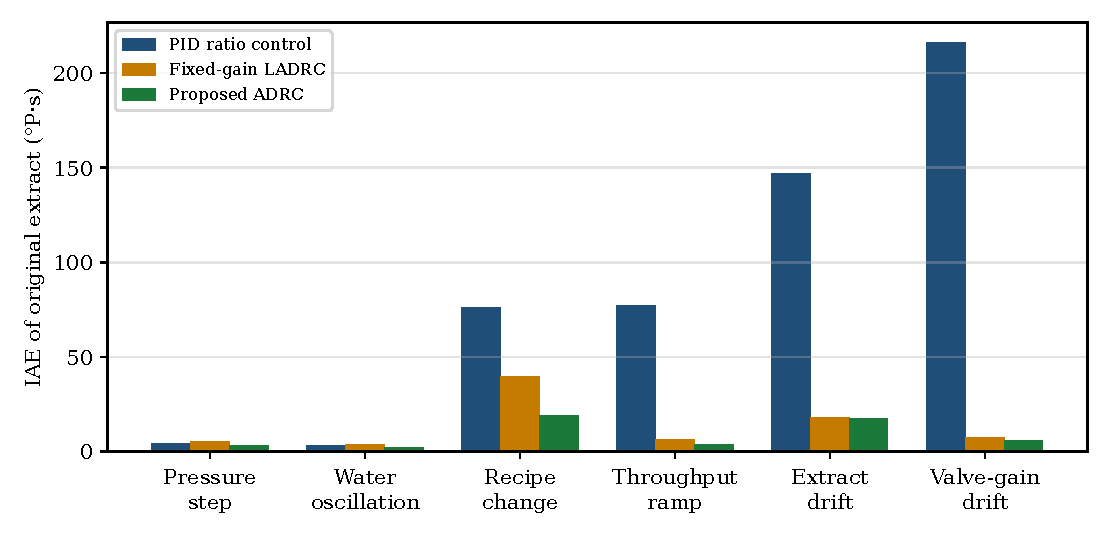
\includegraphics[width=\textwidth]{iae_bars.pdf}
\caption{Integrated absolute error of original extract on each disturbance window.}
\label{fig:iae}
\end{figure}

\begin{figure}[htbp]
\centering
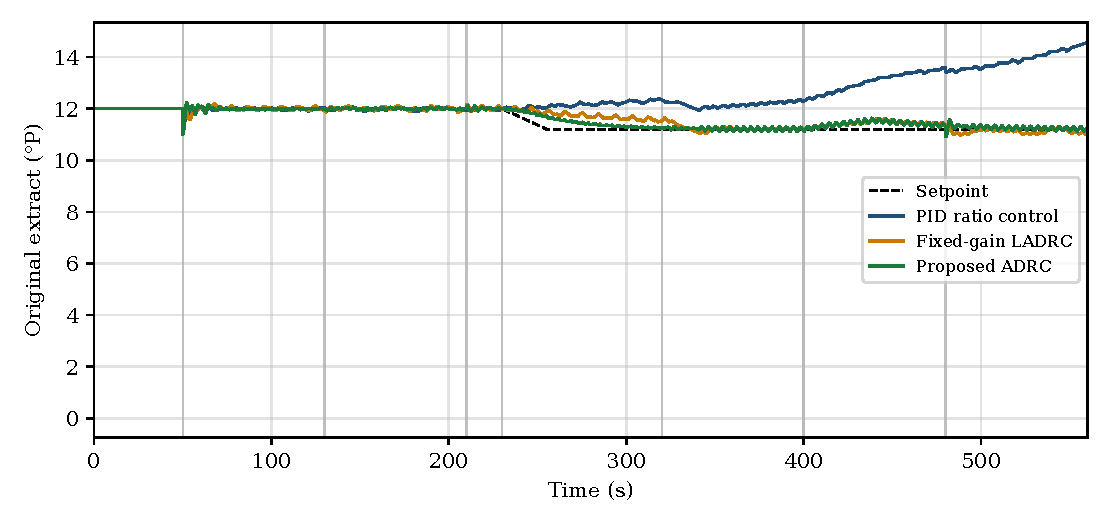
\includegraphics[width=\textwidth]{plato_full.pdf}
\caption{True original extract over the campaign. Vertical lines mark the events of Table~\ref{tab:clock}.}
\label{fig:plato}
\end{figure}

\begin{figure}[htbp]
\centering
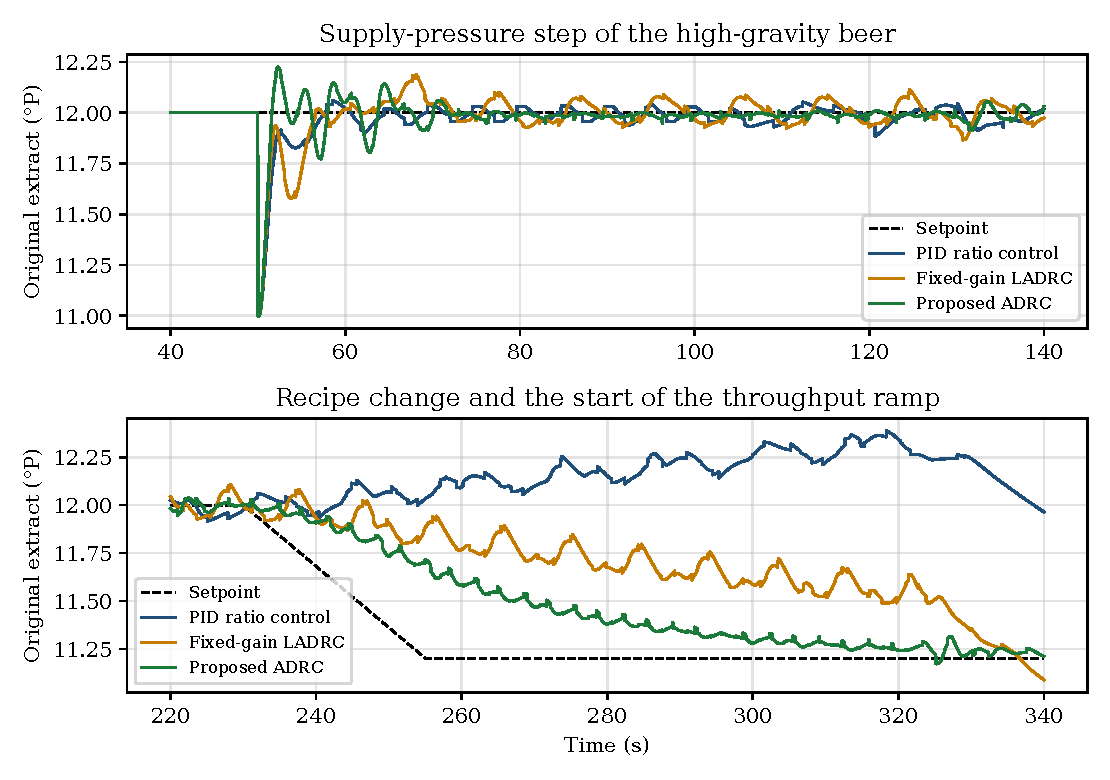
\includegraphics[width=\textwidth]{plato_zoom.pdf}
\caption{Original extract during the beer-supply step and during the brand change.}
\label{fig:zoom}
\end{figure}

\begin{figure}[htbp]
\centering
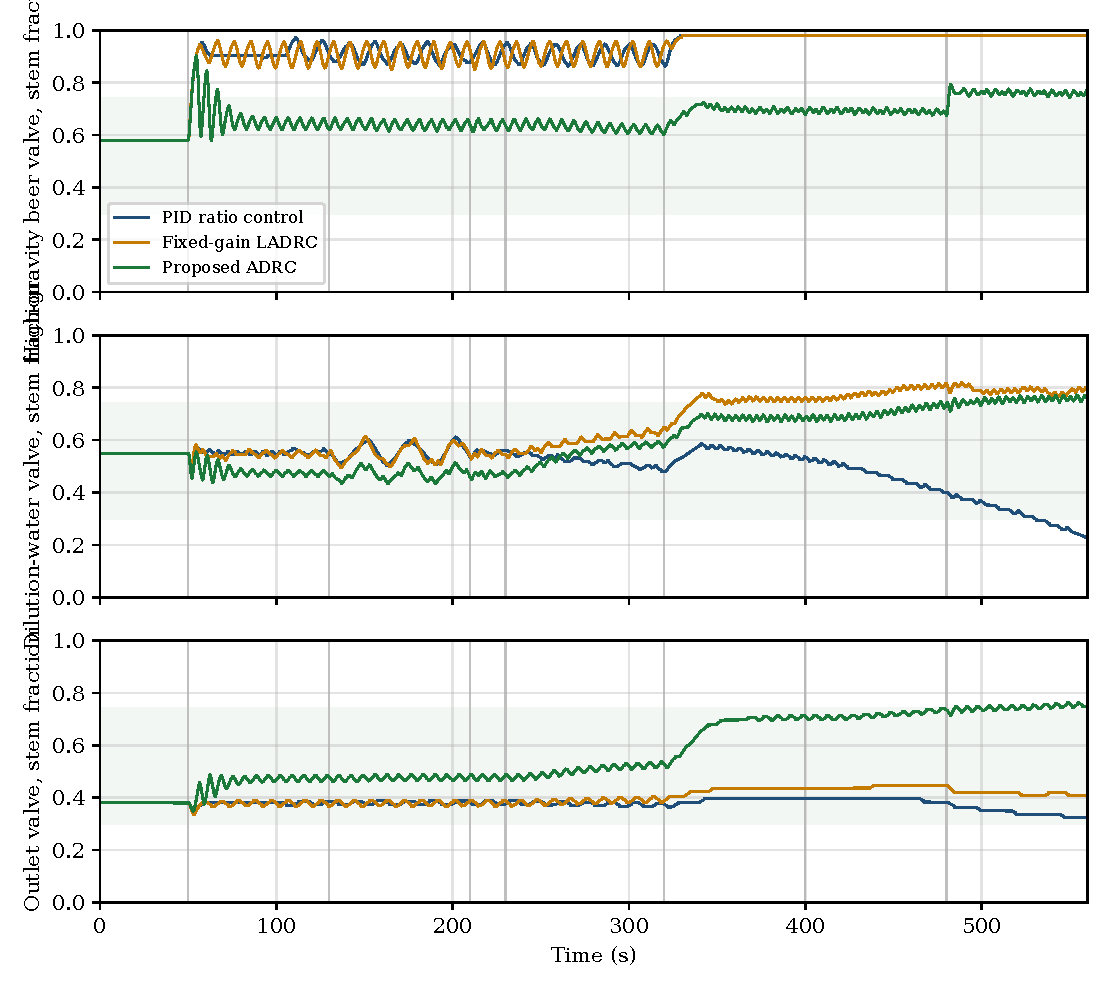
\includegraphics[width=\textwidth]{valves.pdf}
\caption{Stem fractions. The shaded band is the linear window $[0.30,0.74]$ in which the header bandwidth stays at its base value.}
\label{fig:valves}
\end{figure}

\subsection{Supply-pressure step}

On the window from \SI{50}{s} to \SI{130}{s} the extract integrals are $4.03$, $5.53$ and $3.36\ \degP\cdot\mathrm{s}$ for proportional--integral control, fixed-gain active disturbance rejection and the proposed pair. Settling to $\pm 0.05\degP$ takes \SI{72}{s} for proportional--integral control and \SI{46}{s} for the proposed pair. The fixed-gain observer does not stay inside the band before the next event. Its beer-flow integral on this window is \SI{14.0}{\cubic\metre\per\hour\second}, against \SI{12.8}{} for the proposed controller and \SI{7.7}{} for proportional--integral control. The proportional--integral flow loop is stiff at the old gain and so it recovers flow quickly, at the price of driving the beer stem to $0.91$. The proposed stem opens only to about $0.68$ and the header falls to \SI{1.85}{\barg}, which is the coordinator paying for that restraint with outlet travel of $1.02$ on the window, against $0.41$ and $0.12$ for the baselines.

Figure~\ref{fig:pressures} shows the supplies and the header. The proposed header setpoint leaves \SI{2.40}{\barg} within a few seconds of the step and settles near \SI{1.8}{\barg}. Both baselines hold \SI{2.40}{\barg}, as they were asked to. Holding it is what forces the beer valve up the installed curve of Figure~\ref{fig:installed}. The fixed-gain observer is slightly worse than proportional--integral control on this particular window because its $b_0$ is now too large for the reduced drop: the cancellation in \eqref{eq:ladrc-u} overstates the gain, the effective bandwidth falls, and the flow recovery is sluggish. The scheduled $b_{0,h}$ of \eqref{eq:b0h} removes that particular mistake. The remaining advantage of the proposed pair on the extract integral is the soft sensor, which trims $R$ from $\hat{P}$ while the baselines are still waiting for $P_{\mathrm{meas}}$.

\begin{figure}[htbp]
\centering
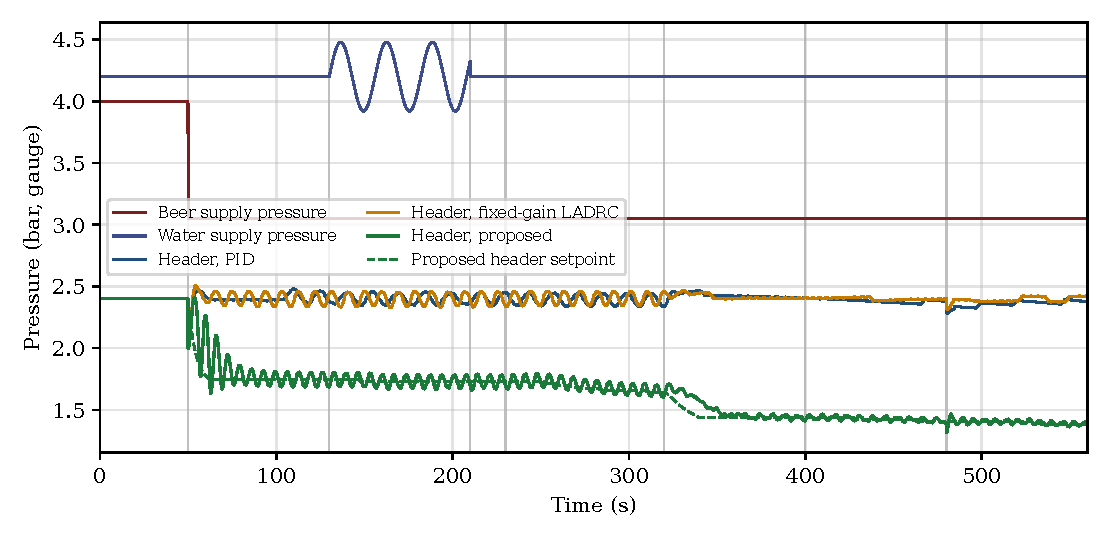
\includegraphics[width=\textwidth]{pressures.pdf}
\caption{Supply pressures and blend-header pressure. The proposed header setpoint is lowered after the beer-supply step so that the inlet valves keep their pressure drop.}
\label{fig:pressures}
\end{figure}

\subsection{Water-supply oscillation}

From \SI{130}{s} to \SI{210}{s} the water supply oscillates with amplitude \SI{0.28}{\barg}. Peak extract errors are $0.109$, $0.140$ and $0.086\degP$. Time spent outside $\pm 0.05\degP$ is \SI{30}{s}, \SI{32}{s} and \SI{7.8}{s}. The proposed beer-flow integral on the window is $4.89$, against $10.2$ for the fixed-gain observer and $6.62$ for proportional--integral control.

The oscillation is a measured disturbance. It enters $G_{ww}$ through $\Delta p_w$ on the sample it occurs. The water-loop $b_{0,w}$ therefore moves with the oscillation, lagged by the \SI{2.5}{s} gain filter, and the command partially anticipates the gain change. The fixed-gain observer must put the whole oscillation into $z_2$. It does reject it, which is why the extract error stays near a tenth of a degree rather than growing, but the rejection is late by a fraction of the observer bandwidth and the peak is the largest of the three. Proportional--integral control has no observer and rejects the oscillation by the integral state, with a peak between the other two. The header loop of the proposed controller moves as well, because the coordinator sees a changing water supply; the outlet travel on the window is $0.55$, and the stem plot shows a slow modulation rather than a copy of the \SI{26}{s} sine at high amplitude.

\subsection{Brand change}

The setpoint ramp from \SI{12.0}{\plato} to \SI{11.2}{\plato} occupies \SIrange{230}{255}{s}. The window used for the indices runs to \SI{320}{s}, so it includes the ramp and \SI{65}{s} of settling. Extract integrals are $76.2$, $39.6$ and $19.2\ \degP\cdot\mathrm{s}$. The proposed controller re-enters the $\pm 0.05\degP$ band \SI{89}{s} after the start of the window, that is about \SI{64}{s} after the ramp has finished. Neither baseline has settled when the throughput ramp begins.

This is the delay comparison. The required ratio change is from $0.338$ to $0.434$, a water-flow change of about \SI{0.72}{\cubic\metre\per\hour} at the pre-ramp beer flow. The soft sensor sees the extract move as soon as the water flow moves, and the extract bandwidth $0.12\ \si{\radian\per\second}$ finishes most of the change inside a minute. The analyser-based observer at $0.055\ \si{\radian\per\second}$, behind eleven seconds of delay, is still \SI{0.48}{\plato} high at \SI{280}{s} ($11.68$ against $11.20$). Proportional--integral control on the analyser is further behind, at $12.15$. Figure~\ref{fig:zoom} shows the three trajectories: the proposed extract follows the ramp with a lag of a few seconds, and the baselines follow a delayed and filtered copy of it.

The peak error of the proposed controller on this window is \SI{0.51}{\plato}, which occurs during the ramp itself, when the setpoint is moving faster than $\omega_{c,R}$ can follow. That peak is the cost of keeping the extract loop slower than the flow loops. Raising $\omega_{c,R}$ toward the flow bandwidth reduces the ramp lag and couples the extract loop into the water valve strongly enough to disturb the beer flow. The value in Table~\ref{tab:bw} is the compromise the build was tuned to, not the lowest integral achievable by a faster unstable loop.

\subsection{Throughput ramp under the reduced supply}

From \SI{320}{s} the beer-flow setpoint rises to \SI{9}{\cubic\metre\per\hour} while the beer supply is still \SI{3.05}{\barg}. This is the joint authority test. Beer-flow integrals on \SIrange{320}{400}{s} are $74.9$, $69.3$ and $4.83\ \si{\cubic\metre\per\hour\second}$. Extract integrals are $77.3$, $6.25$ and $3.68\ \degP\cdot\mathrm{s}$.

Figure~\ref{fig:flows} shows why the baseline flow integrals are large. Both baseline beer valves reach the open limit near $0.98$ and the delivered beer flow stays near \SI{8}{\cubic\metre\per\hour} or below. The fixed-gain extract controller then holds the extract reasonably well, at the wrong throughput: at \SI{360}{s} its extract is \SI{11.16}{\plato} against \SI{11.20}{\plato}, while its beer flow is \SI{7.96}{\cubic\metre\per\hour}. An extract specification that ignores the production rate would accept this. A blending specification does not, because the bright-beer tank fills slowly and the missing flow is not recovered later in the run. The proposed beer flow at the same instant is \SI{8.90}{\cubic\metre\per\hour} and at \SI{400}{s} it has reached the setpoint. The header is near \SI{1.45}{\barg} and the three stems are near $0.70$.

Proportional--integral control loses the extract as well as the flow on this window. With the beer valve saturated, the ratio $R$ no longer determines the extract, because $Q_h$ is stuck and the water loop is still trying to realise $R Q_h^\star$. The water flow and the beer flow drift apart and the extract at \SI{360}{s} is \SI{12.14}{\plato}, almost a degree above the new brand. The integral state of the extract loop cannot repair a ratio whose beer half is not a free input. This is the concrete form of the statement, in Section~\ref{sec:tech1}, that $z_2$ cannot invent travel beyond the stop.

\begin{figure}[htbp]
\centering
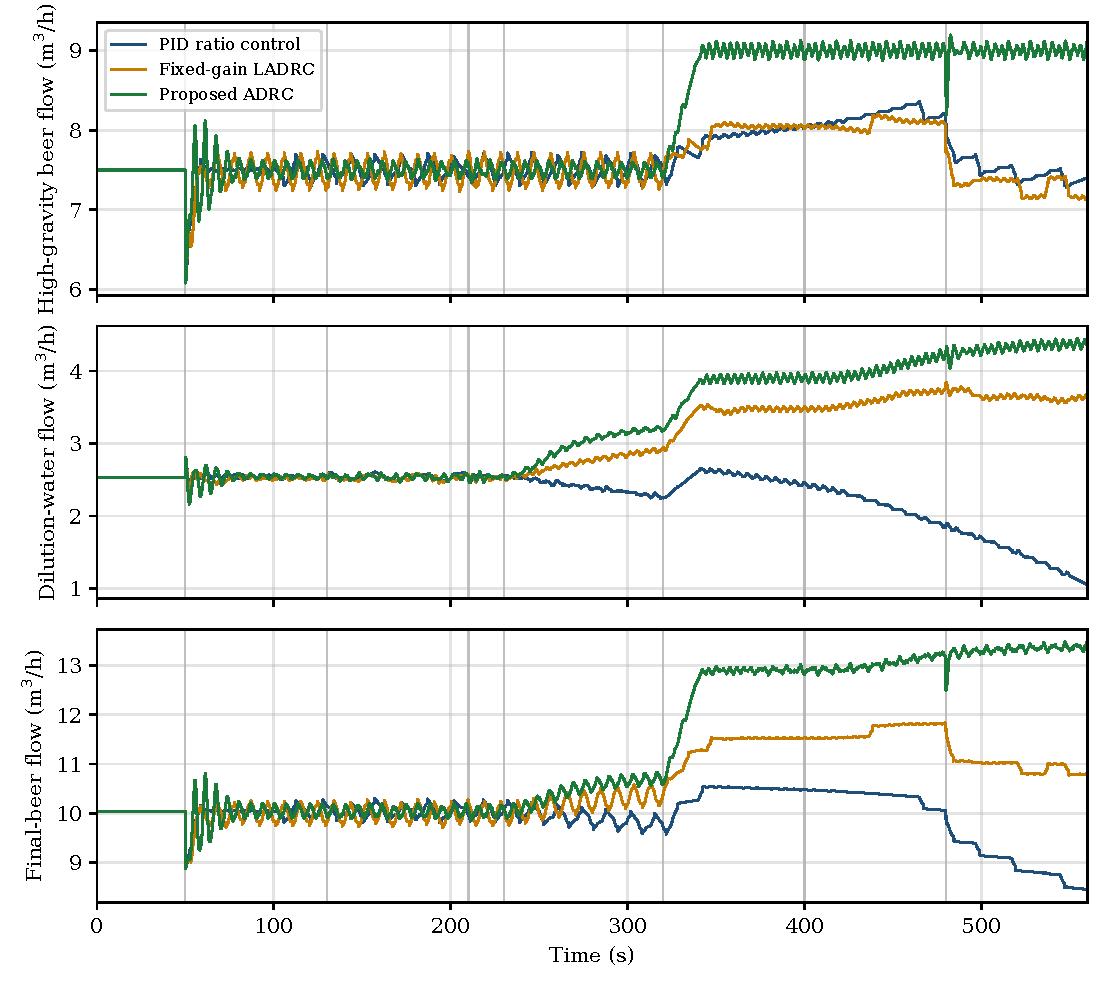
\includegraphics[width=\textwidth]{flows.pdf}
\caption{Volumetric flows. After \SI{320}{s} the beer-flow setpoint is \SI{9}{\cubic\metre\per\hour}. Only the proposed controller reaches it, because the header pressure has been lowered to keep the beer valve inside its travel.}
\label{fig:flows}
\end{figure}

\subsection{Unmeasured drift of the mother-beer extract}

From \SI{400}{s} to \SI{440}{s} the true $P_h$ rises from \SI{16.0}{\plato} to \SI{16.6}{\plato}. The controllers continue to use $16.0$ in any calculation that needs a mother-beer extract. On \SIrange{400}{480}{s} the extract integrals are $147$, $18.0$ and $17.4\ \degP\cdot\mathrm{s}$. The proportional--integral loop, already lost after the throughput ramp, integrates a large offset and finishes the window near \SI{13.3}{\plato}. The two observer-based extract loops both see the analyser. Their integrals are close. The proposed loop has a much smaller beer-flow integral on the same window, $3.99$ against $73.9$, because it is not sitting on the beer-valve stop while it trims water.

Figure~\ref{fig:softsensor} shows the proposed signals. The delayed analyser lags the true extract by about ten seconds. The corrected soft sensor $P_c$ lies between them and is what the extract observer tracks. The bias $b_P$ rises through the drift, as \eqref{eq:bias} requires, and does not run away: the innovation was built so that a bias larger than the true composition error is itself an innovation of the opposite sign. At \SI{450}{s} the true extract is \SI{11.53}{\plato} and at \SI{520}{s}, after the valve-wear transient, it is \SI{11.33}{\plato} against the setpoint \SI{11.20}{\plato}. The residual is the \SI{28}{s} bias lag still finishing its correction, not a frozen offset. A shorter $T_b$ reduces this residual and, in earlier builds of the same plant, produced an overshoot past the setpoint of several tenths of a degree. The recorded value is the slower, non-overshooting choice.

The fixed-gain extract loop ends the campaign closer to the setpoint on extract alone, at \SI{11.16}{\plato}. It does so at a beer flow of \SI{7.38}{\cubic\metre\per\hour}. The two numbers must be read together. A composition controller that is allowed to abandon the production rate has an easier composition problem, because it has an extra free input, the flow it chose not to deliver. The proposed controller is required to deliver both, and at \SI{520}{s} it delivers \SI{9.06}{\cubic\metre\per\hour} at \SI{11.33}{\plato}, with the bias still closing.

\begin{figure}[htbp]
\centering
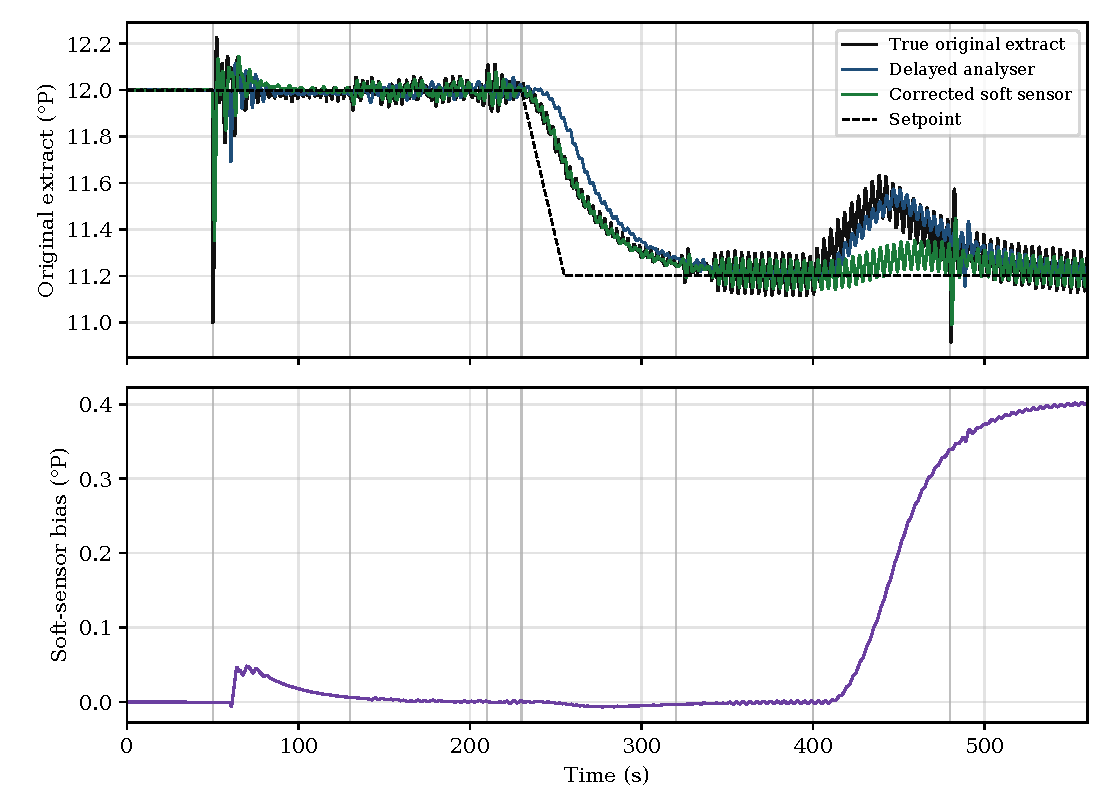
\includegraphics[width=\textwidth]{softsensor.pdf}
\caption{Proposed extract signals. The analyser lags the mix-point extract. The bias is the analyser correction applied to the mass-balance soft sensor.}
\label{fig:softsensor}
\end{figure}

\subsection{Loss of beer-valve capacity}

At \SI{480}{s} the beer $K_v$ falls by ten percent. Nothing in the controller is told. On \SIrange{480}{560}{s} the beer-flow integrals are $121$, $135$ and $4.60\ \si{\cubic\metre\per\hour\second}$. Extract integrals are $216$, $7.22$ and $6.05\ \degP\cdot\mathrm{s}$.

The installed-gain formula does not use $K_v$. It uses the flow that the weakened valve is actually passing. Within the \SI{2.5}{s} gain filter, $b_{0,h}$ falls and the beer command opens. The stem moves from about $0.70$ to $0.77$, the flow returns to \SI{9.06}{\cubic\metre\per\hour}, and the extract excursion peaks at \SI{0.38}{\plato}. The baseline beer valves are already at the stop, so a further loss of $K_v$ cannot be met by stem movement. Their beer-flow integrals on this window are the integrals of a flow that is stuck near \SI{7.3}{\cubic\metre\per\hour} against a setpoint of \SI{9}{\cubic\metre\per\hour}. Proportional--integral extract control drives the water valve shut in an attempt to raise the extract, and the extract reaches \SI{13.8}{\plato}. The fixed-gain extract observer, slower and delayed, holds the extract near the setpoint by a water flow that happens to match the reduced beer flow, and abandons the rate.

Figure~\ref{fig:bandwidth} shows the scheduled header bandwidth. It stays at the base value $0.20\ \si{\radian\per\second}$ for most of the campaign, because the coordinator keeps the stems inside the window that \eqref{eq:schedule} treats as acceptable. It rises only near the end, when the beer stem passes $0.74$ during the $K_v$ loss. The schedule is therefore a guard rather than a permanent retuning. A plant that needed the ceiling bandwidth for long intervals would be a plant whose outlet valve was too small for the requested flow, and the right response would be a larger $K_{v,b}$, not a faster observer. The outlet valve in Table~\ref{tab:design} was sized at stem $0.38$ precisely so that this guard would be enough.

\begin{figure}[htbp]
\centering
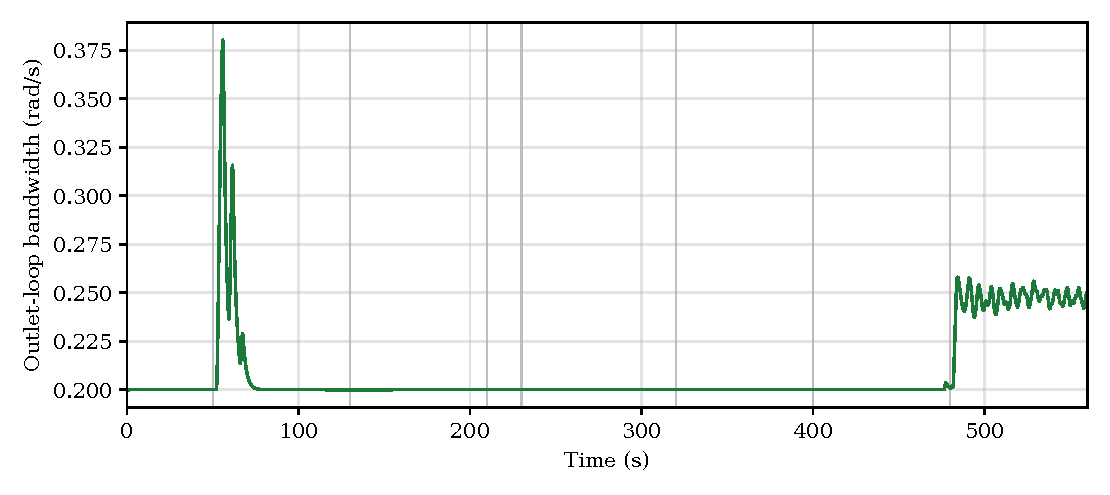
\includegraphics[width=\textwidth]{bandwidth.pdf}
\caption{Scheduled bandwidth of the outlet-valve controller. The base value is held while the inlet stems remain in the linear window.}
\label{fig:bandwidth}
\end{figure}

\subsection{Reading the baseline that looks quiet}

Proportional--integral control has the smallest valve travel in Table~\ref{tab:overall}. For the outlet valve the travel is $0.61$ over \SI{560}{s}. The stem plots show why. The outlet valve barely leaves its initial stick band, because the header error at a fixed setpoint of \SI{2.40}{\barg} stays near the threshold of the stick band for long intervals, and the inlet valves do the rejecting. Quiet travel here is an unused actuator. The extract and flow integrals are the cost of leaving it unused.

Fixed-gain active disturbance rejection is the stronger baseline, and on extract alone it is already an order of magnitude better than proportional--integral control. The bandwidth parameterisation, the consistent initial state and the observer anti-wind-up are doing the work Han and Gao described \cite{han2009pid,gao2003scaling,herbst2013simulative}. The campaign shows where that controller stops. It stops when the gain inside $b_0$ is wrong for a long time, and it stops when the only way to keep the gain right is to move a valve that the controller was not told to move. Those are the two gaps Chapter~\ref{ch:review} identified, and they are the two gaps the indices assign to the proposed pair: the flow integral falls from $316$ to $37.5$ because the header setpoint restores the drop, and the extract integral falls from $81.4$ to $52.4$ because the soft sensor removes the analyser delay from the brand change.

\subsection{What the estimation does not claim}

The plant is the design model, integrated at \SI{10}{ms}, with the disturbances of Table~\ref{tab:clock} and one noise draw. It does not include a pump curve, a bright-beer tank level, dissolved-oxygen dynamics, or the hysteresis of a valve that has been in service for years beyond the stick band used here \cite{choudhury2008stiction,jelali2010stiction}. A valve with a stick band of several percent would change the travel numbers and might force a lower $\omega_o$. The build acceptance tests of Section~\ref{sec:build} would still be the right first check on a factory skid: design-point flows, and the initial flow derivative after a small stem step, which confirms $b_0$.

The proportional--integral and fixed-gain observers were tuned by the same rules as the proposed loops, at the design point, and were not retuned against the later disturbances. Retuning the baselines at the low supply pressure would improve their behaviour at that pressure and worsen it at the design pressure. The proposed $b_0(t)$ is the retuning, done by the measurements, which is the comparison the technique is meant to win. A retuning that uses knowledge of the scenario clock would not be an admissible controller.

No index in this chapter is a flavour index. Stewart's review of high-gravity brewing records foam and ester differences that a correct original extract does not remove \cite{stewart2010highgravity,briggs2004brewing,boulton2001yeast}. The techniques keep the extract and the flow at the values the brand and the production plan specify. They do not enlarge the set of mother beers the brewery can ferment.

Within those limits the estimation is unambiguous. On a line with three linear valves, measured speeds and measured pressures, the pressure-manifold gain and the valve-authority setpoint are what keep the beer valve off the stop, and the mass-balance soft sensor with a delayed bias is what lets the extract loop run at the cascade bandwidth rather than at the delay bandwidth. The numerical values are those of Table~\ref{tab:overall}.

\subsection{Window table}

Table~\ref{tab:windows} repeats the indices at the resolution of Table~\ref{tab:clock}. It is the table a reader should use to check any sentence in this section. The steady window is the noise floor. Every later window is one disturbance, except that the supply pressure remains low after \SI{50}{s}, so the throughput window and the windows after it are joint tests with that low supply.

\begin{table}[htbp]
\centering
\caption{Extract IAE in $\degP\cdot\mathrm{s}$ and beer-flow IAE in \si{\cubic\metre\per\hour\second}, by window.}
\label{tab:windows}
\begin{tabular}{@{}lrrrrrr@{}}
\toprule
 & \multicolumn{3}{c}{Extract IAE} & \multicolumn{3}{c}{Beer-flow IAE} \\
\cmidrule(lr){2-4}\cmidrule(lr){5-7}
Window & PID & LADRC & Prop. & PID & LADRC & Prop. \\
\midrule
Steady & 0.005 & 0.005 & 0.005 & 0.007 & 0.007 & 0.007 \\
Pressure step & 4.03 & 5.53 & 3.36 & 7.71 & 14.0 & 12.8 \\
Water oscillation & 3.40 & 3.64 & 2.02 & 6.62 & 10.2 & 4.89 \\
Brand change & 76.2 & 39.6 & 19.2 & 8.73 & 11.3 & 5.08 \\
Throughput & 77.3 & 6.25 & 3.68 & 74.9 & 69.3 & 4.83 \\
Extract drift & 147 & 18.0 & 17.4 & 65.8 & 73.9 & 3.99 \\
Valve wear & 216 & 7.22 & 6.05 & 121 & 135 & 4.60 \\
\bottomrule
\end{tabular}
\end{table}

Two columns of this table carry the claim of the thesis. The beer-flow column from the throughput window onward is where valve authority is visible: the proposed integral stays near \SI{4}{\cubic\metre\per\hour\second} on an \SI{80}{s} window, which is a mean absolute error of about \SI{0.05}{\cubic\metre\per\hour}, while both baselines sit near \SI{70}{\cubic\metre\per\hour\second} or above, a mean error of about \SI{1}{\cubic\metre\per\hour} on a setpoint of \SI{9}{\cubic\metre\per\hour}. The extract column on the brand-change window is where the soft sensor is visible: the proposed integral is half the fixed-gain observer and a quarter of the proportional--integral loop. On the extract-drift window the two observers are close, and the proportional--integral loop has already been lost by the saturated beer valve. The techniques do different jobs, and the table shows both jobs rather than a single average that could hide one of them.

\subsection{Mean errors}

Dividing an integral by the length of the window gives a mean absolute error, which is easier to compare with the tolerance \SI{0.05}{\plato}. On the brand-change window of \SI{90}{s} the proposed mean absolute extract error is $19.2/90 = \SI{0.21}{\plato}$, most of it accumulated while the setpoint is still moving. On the pressure-step window of \SI{80}{s} it is $3.36/80 = \SI{0.042}{\plato}$, inside the tolerance on average, with the settling time of \SI{46}{s} saying that the first half of the window contains the excursion and the second half does not. The fixed-gain observer on that window averages $5.53/80 = \SI{0.069}{\plato}$ and does not settle. Proportional--integral control averages $4.03/80 = \SI{0.050}{\plato}$ and settles in \SI{72}{s}, with the beer stem already at $0.91$. Average extract error alone would rank proportional--integral control close to the proposed controller on the supply step. The stem and the later throughput window are what separate them: the proportional--integral loop has spent the authority the later ramp needed.

On the full run the proposed mean absolute extract error is $52.4/560 = \SI{0.094}{\plato}$ and the mean absolute beer-flow error is $37.5/560 = \SI{0.067}{\cubic\metre\per\hour}$. The fixed-gain observer's means are \SI{0.145}{\plato} and \SI{0.57}{\cubic\metre\per\hour}. The proportional--integral means are \SI{0.94}{\plato} and \SI{0.51}{\cubic\metre\per\hour}. The flow means of the two baselines are similar because both lose the beer valve for the same physical reason. Their extract means differ because the observer still trims water from the analyser and the proportional--integral loop, once the beer flow is stuck, trims water from a ratio that no longer describes the plant.

\subsection{Build parameters collected for reproduction}

A later estimation can reproduce the campaign from the following list, together with the equations of Chapter~\ref{ch:design}. Step \SI{10}{ms}. Positioner time constant \SI{2.4}{s}, stick release at stem error $0.014$, recapture at $0.005$. Command filter \SI{0.40}{s}. Measurement filter \SI{0.30}{s}. Gain filter \SI{2.5}{s}. Header-setpoint lag \SI{4}{s} outside a dead zone of \SI{0.04}{\barg}. Bias time \SI{28}{s}, bias limit $\pm 1.5\degP$. Pipe length \SI{14}{m}, analyser lag \SI{1.2}{s}. Noise standard deviations as in Section~\ref{sec:build}, generator seed fixed so that the three controllers share one draw. Flow limits on the stem command $[0.02,0.98]$, ratio limits $[0.08,0.85]$. Bandwidths as in Table~\ref{tab:bw}. Proportional--integral numbers as in Section~\ref{sec:build}. The header root is Brent's method on \eqref{eq:node}. Nothing in the campaign is filtered after the fact: the integrals use the true mix-point extract and the true beer flow at the controller sample rate.

\FloatBarrier
\typeout{END CHAPTER 3 ON PAGE \thepage}


\bibliographystyle{IEEEtran}
\bibliography{refs}

\end{document}
